\documentclass[12pt,a4paper,oneside]{report}

% --- Packages ---
\usepackage[utf8]{inputenc}
\usepackage[T1]{fontenc}
\usepackage[margin=1in]{geometry}
\geometry{margin=1.5cm}
\usepackage{graphicx}
\usepackage{amsmath}
\usepackage{hyperref}
\usepackage{titlesec}
\usepackage{setspace}
\usepackage{booktabs}
\usepackage[margin=1in]{geometry}
\usepackage{tikz}
\usepackage{pgfplots}
\pgfplotsset{compat=1.18}
\usetikzlibrary{arrows.meta, shapes.geometric, positioning, fit, backgrounds, calc}
\usepackage{amssymb}
\usepackage{array}
\usepackage{multirow}
\usepackage{xcolor}


% ================= TITLE PAGE =================
\begin{document}

\begin{titlepage}
    \centering

    % --- Logos and Country Text ---
    \begin{minipage}{0.25\textwidth}
        \centering
        \includegraphics[width=3cm]{university logo.jpg}
    \end{minipage}
    \hfill
    \begin{minipage}{0.45\textwidth}
        \centering
        {\Large \textbf{People’s Democratic Republic of Algeria}}\\[0.2cm]
        {\Large Ministry of Higher Education and Scientific Research}
    \end{minipage}
    \hfill
    \begin{minipage}{0.25\textwidth}
        \centering
        \includegraphics[width=3cm]{university logo.jpg}
    \end{minipage}

    \vspace{1.2cm}

    % --- University Info ---
    {\Large \textbf{Bouira University}}\\[0.3cm]
    {\large Faculty of Exact Sciences}\\
    {\large Department of Computer Science}

    \vspace{1.5cm}

     % --- Degree ---
    {\Large \textbf{Master Thesis}}
    
    \vspace{0.5cm}
    % --- Top Divider ---
    \rule{\textwidth}{1.2pt}

    \vspace{0.8cm}

    % --- Thesis Title ---
    {\LARGE \textbf{Robust Steganography Techniques for Data Tampering Resilience}}

    \vspace{0.8cm}

    % --- Bottom Divider ---
    \rule{\textwidth}{1.2pt}

    \vspace{1.5cm}

    % --- Students & Supervisor ---
    \begin{flushleft}
        \textbf{Submitted by:}\\[0.2cm]
        Abid Akram\\
        Tahraoui Mustapha\\[0.8cm]

        \textbf{Supervised by:}\\[0.2cm]
        Dr. Benaissi Sellami
    \end{flushleft}

    \vfill

    % --- Footer ---
    {\large Submitted in partial fulfillment of the requirements for the degree of}\\[0.2cm]
    {\large \textbf{Master in Computer Science}}\\[0.6cm]
    {\large Academic Year: 2025 -- 2026}

\end{titlepage}

% =================================================
\tableofcontents
\newpage
\listoffigures
% =================================================
% =========================
% Thesis Plan
% =========================

\chapter{Introduction}

\section{General Background} In contrast to cryptography, which focuses on protecting the content of a message by transforming it into an unreadable form, steganography aims to conceal the very existence of communication. While digital watermarking shares similarities with steganography, it is primarily designed for ownership verification and copyright protection rather than covert communication. Robust steganography lies at the intersection of these domains, seeking to maintain hidden communication while ensuring resistance to intentional or unintentional image modifications.

In real-world digital environments, images rarely remain unchanged after distribution. Common platforms such as social media networks, cloud storage services, and messaging applications routinely apply operations including lossy compression, resizing, filtering, and format conversion. These automatic transformations pose a significant threat to traditional steganographic techniques, which are often designed under ideal transmission assumptions. As a result, the development of steganographic systems capable of surviving such uncontrolled and hostile processing environments has become an essential research challenge.


Steganography is the art and science of invisible communication, achieved by concealing information within other digital content in such a way that the existence of the hidden message remains undetectable. The term steganography is derived from the Greek words stegos, meaning “cover,” and graphia, meaning “writing,” and is commonly interpreted as “covered writing.”\cite{moerland2005steganography}. In the context of image steganography, secret information is embedded exclusively within digital images, which serve as the cover medium for hidden communication.

\section{Problem Statement}
From the analysis above, the core challenges addressed in this work can be summarized as follows:

\begin{itemize}
    \item Existing steganographic methods exhibit high fragility when subjected to common signal processing operations such as compression, noise addition, and filtering, resulting in partial or complete loss of embedded information.
    
    \item Geometric transformations, including cropping and resizing, introduce spatial desynchronization between the embedding and extraction processes, severely limiting reliable data recovery.
    
    \item Most current approaches prioritize imperceptibility while neglecting the survivability of the hidden payload under compound or severe distortions.
    
    \item The majority of embedding strategies focus on protecting embedding locations rather than enabling resilience or reconstruction of the hidden message itself.
\end{itemize}

These limitations highlight the need for a steganographic framework that shifts the design focus from invisibility-centered embedding toward payload-oriented survivability, enabling partial recovery and reliable communication in hostile and uncontrolled digital environments.


\section{Research Objectives}

The primary objective of this research is to address the limitations of conventional image steganography techniques by prioritizing the survivability of hidden data under adverse and uncontrolled image degradation. Rather than focusing exclusively on high-capacity or imperceptible embedding, this work aims to enhance the resilience of the embedded payload against both signal processing and geometric distortions.

The specific objectives of this thesis are as follows:

\begin{itemize}
    \item To design a robust steganographic framework that improves the survivability of hidden information under severe and compound image degradations.
    
    \item To structure the secret payload into interconnected fragments that enable partial data recovery when segments of the stego-image are lost or corrupted.
    
    \item To distribute embedded message fragments across stable image regions and multiple transform domains in order to reduce the impact of localized tampering.
    
    \item To develop an extraction and reconstruction strategy capable of recovering usable information even in the presence of spatial misalignment and partial data loss.
    
    \item To evaluate the proposed framework using standard image quality and robustness metrics, including PSNR \cite{gonzalez2008digital} and Bit Error Rate (BER) \cite{proakis2008digital}, under realistic attack scenarios.
\end{itemize}

\section{Scope and Contributions}

This research focuses on robust data hiding in digital images, with particular emphasis on improving the survivability of hidden information under common image degradation and tampering scenarios. The scope of this work is limited to still images and does not address steganography in video, audio, or real-time streaming media. Furthermore, the proposed framework does not aim to maximize payload capacity, but instead prioritizes reliable data recovery under adverse conditions.

The study assumes that image degradation may occur due to both unintentional processing (such as compression and resizing) and intentional tampering (such as cropping or localized modification). However, the framework does not guarantee successful recovery under all extreme or adversarial scenarios, particularly in cases of complete image destruction or aggressive multi-stage attacks.

The main contributions of this thesis can be summarized as follows:

\begin{itemize}
    \item Proposing a robustness-oriented steganographic framework that emphasizes payload survivability rather than solely protecting embedding locations.
    
    \item Introducing a structured message fragmentation strategy that enables partial reconstruction of the hidden data when portions of the stego-image are lost or corrupted.
    
    \item Designing a multi-domain embedding strategy that distributes message fragments across different image regions to reduce sensitivity to localized distortions.
    
    \item Developing an extraction and reconstruction mechanism capable of recovering meaningful information under spatial misalignment and partial data loss.
    
    \item Providing an experimental evaluation of the proposed framework under realistic signal processing and geometric attack scenarios.
\end{itemize}


\section{Thesis Organization}

The remainder of this thesis is organized as follows. Chapter~2 presents a comprehensive review of existing steganographic techniques, with particular emphasis on robustness-oriented approaches and their limitations under image degradation and tampering. Chapter~3 introduces the proposed robust steganography framework, detailing its design principles, message structuring strategy, and embedding and extraction mechanisms. Chapter~4 describes the implementation details, experimental setup, datasets, attack models, and evaluation metrics used in this study. Chapter~5 presents and discusses the experimental results, including imperceptibility and robustness analyses as well as comparative evaluations with classical methods. Finally, Chapter~6 concludes the thesis by summarizing the main findings, discussing limitations, and outlining directions for future research.

% =========================

\chapter{Literature Review}

\section{Fundamentals of Image Steganography}
Image steganography refers to techniques that embed secret information within digital images while preserving the visual appearance of the carrier. In contrast to introductory definitions presented earlier, this chapter focuses on how steganographic systems are modeled, evaluated, and constrained in practical scenarios. A widely adopted theoretical model is the prisoner's problem, in which the security of a steganographic system depends on the inability of an adversary to statistically distinguish between cover images and stego-images \cite{morkel2005overview}. This model emphasizes that effective steganography must balance invisibility with functional robustness under realistic transmission conditions.

\subsection{Imperceptibility, Capacity, and Robustness Trade-off}

The efficacy of the image steganography system is inevitably limited by the trade-off between the following two factors:
between three key performance criteria: imperceptibility, payload capacity, and robustness. These
Three properties are necessarily interconnected so that enhancement in one area will result in improvement in other areas as well.
decline in at least one of the others. This pattern is often represented in a triangular relationship:
This represents a trade-off and is one of the main challenges in designing a steganographic system \cite{Fridrich2012}.

\begin{itemize}
\item \textbf{Imperceptibility} refers to the degree to which a stego-image remains visually and statistically indistinguishable from the corresponding cover image. Imperceptibility is a crucial factor in steganography
to avoid being detected either by human observers or statistical steganalysis algorithms. Methods which
Agressively embedded data could introduce artifacts that affect either the statistical distribution or signal quality. For example, data that has
risk of detection \cite{provos2003hide}.

\item \textbf{Payload capacity }denotes the amount of secret information that can be embedded within a cover image. While higher capacity improves communication efficiency, it typically requires stronger or more frequent modifications to the image content, which negatively impacts imperceptibility and increases vulnerability to image processing operations. Consequently, high-capacity embedding schemes often sacrifice robustness in order to maximize payload \cite{johnson1998exploring}.

\item \textbf{Robustness} describes the ability of the embedded information to survive image degradation caused by signal processing operations or intentional attacks. Robust steganographic schemes are designed to withstand distortions such as compression, noise addition, filtering, and geometric transformations. Achieving robustness usually requires redundancy, structured embedding, or the use of stable image components, which in turn reduces the effective payload capacity \cite{cox2007digital}.
\end{itemize}

\begin{figure}[htbp]
    \centering
    \includegraphics[width=0.9\textwidth]{triangle.png}
    \caption{Steganography Trilemma: Three Competing Goals}
    \label{fig:trilemma}
\end{figure}

In the context of robust steganography, robustness is frequently prioritized over capacity, particularly in applications where data recovery is more critical than transmission efficiency. As a result, many robust systems intentionally operate at lower payload rates to ensure reliable extraction under adverse conditions. Balancing these three competing objectives remains a key research challenge and motivates the exploration of resilience-oriented steganographic frameworks.

\section{Spatial Domain Techniques}

Spatial domain approaches embed the secret by directly modifying the intensities of pixels.
the cover image. Among the methods, one can distinguish LSB substitution and its variants
are the most studied families due to their simplicity and low computational complexity.
High embedding capacity\cite{johnson1998exploring}. In LSB-based methods, the least significant bits of pixel values are
changed to convey secret information, leading to less than ideally perceivable distortion.

Spatial domain techniques, despite all their advantages, suffer from some serious drawbacks in terms of
robustness. Since the embedding procedure acts directly on pixel values, the hidden data is
highly susceptible under common image processing manipulations. Even light lossy compression, noise addition,
Filtering irreversibly destroys some fractional bits of the least significant bits, and the result can be a partial or complete loss.
of the embedded message\cite{provos2003hide}. Hence, most spatial domain methods are unsuitable for applications that require robustness against image degradation or tampering as a main constraint.

\subsection{Transform Domain Techniques}

According to the Discrete Cosine Transform (DCT), the DCT is an example of a method of digital image steganography that embeds information into the transform domain of a digital image, instead of modifying the pixel intensity values directly. The DCT takes advantage of the ability of the human visual system to be less sensitive to different spectral components in the image, particularly when working in the frequency or multi-resolution space\cite{cox2007digital}.

\subsection{Discrete Cosine Transform (DCT)-Based Steganography}

The Discrete Cosine Transform (DCT) is a fundamental transform-domain technique widely used in image steganography due to its strong connection with the JPEG compression standard. Unlike spatial-domain approaches that directly modify pixel intensity values, DCT-based steganography embeds secret information within the frequency coefficients of an image. This allows data hiding to exploit the characteristics of the human visual system, which is less sensitive to modifications in certain frequency components \cite{Fridrich2012,cox2007digital}.

\subsubsection{Overview of the DCT Transformation}
The DCT converts spatial image data into a frequency-domain representation. In practice, a grayscale or luminance image is first divided into non-overlapping blocks of size $8 \times 8$ pixels. Each block is then transformed independently using the DCT, resulting in 64 coefficients that represent different spatial frequency components.

The resulting coefficients can be categorized as:
\begin{itemize}
    \item \textbf{Low-frequency coefficients:} Represent the average intensity and coarse image structures.
    \item \textbf{Mid-frequency coefficients:} Represent edges and moderate texture details.
    \item \textbf{High-frequency coefficients:} Represent fine details and noise-like components.
\end{itemize}

\begin{figure}[htbp]
    \centering
    \includegraphics[width=0.6\textwidth]{Frequency-regions-of-88-block-2D-DCT-coefficients.png}
    \caption{DCT coefficient distribution showing low-, mid-, and high-frequency components in an $8 \times 8$ block}
    \label{fig:dct_freq}
\end{figure}

\subsubsection{Embedding Process in DCT-Based Steganography}
    The embedding procedure in DCT-based steganography typically follows a structured sequence of steps:

    \begin{enumerate}
    \item \textbf{Color Space Conversion:}  
    For color images, the RGB image is commonly converted into a luminance-chrominance color space (such as YCbCr). Data embedding is primarily performed in the luminance (Y) channel, as it carries the most perceptual information.

    \paragraph{The YCbCr Components}
    The YCbCr space represents an image through three distinct components:
    \begin{itemize}
        \item \textbf{Y (Luminance):} Represents the brightness information    of the image.
        \item \textbf{Cb (Chroma Blue):} Represents the difference between the blue component and a reference value.
        \item \textbf{Cr (Chroma Red):} Represents the difference between the red component and a reference value.
    \end{itemize}

    \paragraph{Mathematical Transformation}
    The conversion from the digital RGB space to YCbCr is defined by a linear transformation. According to the ITU-R BT.601 standard, the transformation matrix for 8-bit digital signals is expressed as follows:

    \begin{equation}
    \begin{bmatrix} 
    Y \\ 
    Cb \\ 
    Cr 
    \end{bmatrix} = 
    \begin{bmatrix} 
    16 \\ 
    128 \\ 
    128 
    \end{bmatrix} + 
    \begin{bmatrix} 
    65.481 & 128.553 & 24.966 \\ 
    -37.797 & -74.203 & 112.000 \\ 
    112.000 & -93.786 & -18.214 
    \end{bmatrix} 
    \begin{bmatrix} 
    R \\ 
    G \\ 
    B 
    \end{bmatrix}
    \end{equation}

    In a more simplified normalized form, the equations can be written as:

    \begin{align}
    Y &= 0.299R + 0.587G + 0.114B \\
    Cb &= -0.1687R - 0.3313G + 0.5B + 128 \\
    Cr &= 0.5R - 0.4187G - 0.0813B + 128
    \end{align}

    \paragraph{Significance for Robust Steganography}
    By utilizing the YCbCr space, the steganographic algorithm can selectively embed data into the chrominance channels ($Cb$ or $Cr$). Since the Human Visual System (HVS) is less sensitive to these channels, the hidden data can better withstand degradation such as lossy JPEG compression, which typically applies heavier quantization to the chrominance components than to the luminance.


    \item \textbf{Block Division:}  
    The luminance component is divided into non-overlapping $8 \times 8$ blocks to match the JPEG compression structure.


    \begin{figure}[htbp]
    \centering
    \includegraphics[width=0.6\textwidth]{DCT 8 blocks devision.png}
    \caption{DCT deivision image  in an $8 \times 8$ blocks}
    \label{fig:dct_blocks}
\end{figure}

    \item \textbf{DCT Application:}  
    Each block is transformed from the spatial domain to the frequency domain using the DCT, producing a matrix of frequency coefficients.

    \paragraph{Frequency Domain Transformation: Block-Based DCT}

To achieve robustness against signal processing attacks, the proposed framework employs the Discrete Cosine Transform (DCT). The process follows these steps:
\begin{itemize}
    \item Division of the image into $8 \times 8$ pixel blocks.
    \item Application of the DCT to each block.
\end{itemize}

\paragraph{Block Partitioning} % Fixed the 'subsubssubsection' typo
The image channel (e.g., the $Cb$ or $Cr$ component) is first partitioned into non-overlapping blocks of size $N \times N$, where $N=8$. This localization allows the algorithm to handle local image characteristics effectively. Let $f(i, j)$ represent the intensity value at coordinates $(i, j)$ within an $8 \times 8$ block.

\paragraph{Two-Dimensional DCT (2D-DCT)}
For each block, the 2D-DCT is applied to convert the spatial data into the frequency domain. The DCT-II variant is defined as:

\begin{equation}
F(u, v) = \frac{1}{4} C(u) C(v) \sum_{i=0}^{7} \sum_{j=0}^{7} f(i, j) \cos \left[ \frac{(2i+1)u\pi}{16} \right] \cos \left[ \frac{(2j+1)v\pi}{16} \right]
\end{equation}

where $u, v$ are the horizontal and vertical frequencies $u, v \in \{0, 1, \dots, 7\}$, and the normalization factors $C(u)$ and $C(v)$ are defined as:

\begin{equation}
C(k) = 
\begin{cases} 
\frac{1}{\sqrt{2}} & \text{if } k = 0 \\
1 & \text{if } k > 0 
\end{cases}
\end{equation}

    \paragraph{Coefficient Analysis and Robustness}
    The resulting $8 \times 8$ matrix $F(u, v)$ consists of:
    \begin{itemize}
        \item \textbf{DC Coefficient ($F(0,0)$):} Represents the average intensity of the block. While it holds the most energy, modifying it significantly impacts visual quality.
        \item \textbf{AC Coefficients ($F(u,v)$ where $u,v \neq 0$):} Represent higher frequency details.
    \end{itemize}

    \begin{figure}[htbp]
    \centering
    \includegraphics[width=0.4\textwidth]{DC-and-AC-coefficient-on-DCT-Transformation (1).png}
    \caption{DC and AC coefficient on DCT Transformation}
    \label{fig:dct_coefficients}
\end{figure}

    In this research, we target the \textbf{mid-frequency coefficients} for data embedding. High-frequency coefficients are often discarded during lossy compression (quantization), while low-frequency/DC coefficients are too sensitive to changes. Mid-frequency embedding provides an optimal balance between imperceptibility and robustness against tampering.

    \item \textbf{Coefficient Selection:}  
    A predefined set of mid-frequency coefficients is selected for embedding. Low-frequency coefficients are avoided to prevent visible distortion, while high-frequency coefficients are avoided due to their vulnerability to compression.

    \item \textbf{Data Embedding:}  
    Secret bits are embedded by modifying the selected DCT coefficients using techniques such as coefficient quantization, parity modification, or least significant bit alteration of coefficient values.

    \item \textbf{Inverse DCT:}  
    After embedding, the modified coefficients are transformed back into the spatial domain using the inverse DCT to reconstruct the stego-image.
\end{enumerate}

\begin{figure}[htbp]
    \centering
    \includegraphics[width=0.8\textwidth]{dct embeding process.png}
    \caption{Block-based DCT embedding process illustrating transformation, coefficient selection, and inverse transformation.}
    \label{fig:dct_pipeline}
\end{figure}

\paragraph{Extraction Process}
The extraction operation follows the steps in the embedding operation as follows:

\begin{enumerate}
    \item Conversion of the stego-image to the appropriate color space (from the RGB color space to the YCbCr color space).
    \item Aplication of DCT
    \item Identification of the same mid-frequency coefficients used during embedding.
    \item Recovery of the hidden bits based on the coefficient modification rule.
\end{enumerate}

Accurate extraction relies on preserving coefficient alignment and consistent block structure between embedding and extraction.

\subsubsection{DCT Method Benefits}
 compared with the spatial domain method of steganography, DCT offers many benefits:
\begin{itemize}
    \item Robustness against JPEG compression is significantly improved.
    \item and embedding information into the frequency domain allows for better imperceptibility than embedding the hidden message into the spatial domain.
    \item Compatibility with widely used image compression standards.
    \item DCT-based techniques are less vulnerable to simple noise additions.
\end{itemize}

\subsubsection{Limitations and Challenges}
While DCT-based steganography has significant advantages, many disadvantages exist.
\begin{itemize}
    \item  Have limited robustness when exposed to combined or severe geometric distortions such as cropping, resizing, and rotation.
    \item Sensitivity to block misalignment caused by image re-sampling.
    \item The trade-off between payload capacity and robustness is significant.
\end{itemize}

    Although DCT techniques offer substantially increased robustness compared to spatial-domain approaches, DCT alone cannot be relied upon for successful recovery of data under highly adversarial or degradation conditions. \cite{petitcolas1999information}.



\subsection{Discrete Wavelet Transform (DWT)-Based Steganography}

Embedding Data in Images Using DWT-Based Steganography
The Discrete Wavelet Transform (DWT) is a popular method for representing images as a set of wavelet coefficients and DWT is used in image steganography because it is a transform-domain technique that allows for the representation of image information at various resolutions. In contrast to the Discrete Cosine Transform, which processes a fixed-size block of an image, the DWT processes an entire image at all frequency bands and all scales simultaneously, thereby providing a means of implementing image steganography with greater perceptual adaptability and resilience to localized distortions than other techniques  \cite{mallat1999wavelet, chen2006dwt}.

\subsubsection{Overview of the DWT Decomposition}
The DWT works by decomposing an image into a set of frequency sub-bands (subbands) by passing the entire image horizontally and vertically through pairs of low-pass and high-pass filters. After a single level DWT decomposition of an image, we end up with four distinct frequency subbands:
\begin{itemize}
    \item \textbf{LL (Low-Low):} This is the approximation component, which contains the majority of an image's energy and the information regarding its structure.
    \item \textbf{LH (Low-High):} Captures horizontal edge information.
    \item \textbf{HL (High-Low):} Captures vertical edge information.
    \item \textbf{HH (High-High):} Represents diagonal details and fine textures.
\end{itemize}

The LL sub-band can be decomposed again using the same technique (that is recursion). Consequently, the image-represented data set can be represented in a multi-resolution, or hierarchical, manner.

\begin{figure}[htbp]
    \centering
    \includegraphics[width=0.9\textwidth]{dwt decomposition.png}
    \caption{One-level and multi-level DWT decomposition showing LL, LH, HL, and HH sub-bands.}
    \label{fig:dwt_ranges}
\end{figure}

\subsubsection{Embedding Process in DWT-Based Steganography}
The embedding procedure for DWT-based steganography generally consists of the following steps:

\begin{enumerate}
    \item \textbf{Color Space Selection:}  
    an image is first selected for steganography by choosing between either a color space or a luminance (brightness) component. Color images are generally embedded using the luminance component because it maintains a higher perceptual quality than using one of the color channels.

    \item \textbf{Wavelet Decomposition:}  
    DWT Decomposition
After the luminance has been selected, a discrete wavelet transform (DWT) is applied to multiple levels (i.e., level 1, level 2, etc.) in order to obtain multiple subbands corresponding to each level of the decomposition.

    \item \textbf{Sub-band Selection:}  
    The subbands for embedding are generally chosen from the higher or mid-level frequency subbands (e.g., LH, HL, HH).
The low-frequency subband, LL, may cause strong visual effects on the final output image.

    \item \textbf{Coefficient Modification:}  
    Modification of Wavelet Coefficients
Wavelet coefficients are modified to embed secret data, which can be accomplished in various methods (e.g., coefficient quantization, adjusted threshold, or bit-level).


    \item \textbf{Inverse DWT:}  
   After modifying the coefficients of the appropriate subbands, an inverted DWT is performed, returning the steganographic image back to the spatial domain.
\end{enumerate}

\begin{figure}[htbp]
    \centering
    \includegraphics[width=0.9\textwidth]{Dwt process.png}
    \caption{DFT-based embedding process illustrating frequency selection, magnitude modification, and inverse transformation}
    \label{fig:dft_process}
\end{figure}

\subsubsection{Extraction Process}
The process of extracting information through DWT is the reverse of how it was added to the stego-image. The steps for extracting information from the DWT are as follows:

\begin{enumerate}
    \item To use the same wavelet parameters, perform a DWT on the stego-image
    \item Determine which sub-band(s) were used for embedding
    \item Use the coefficient modification rule to determine how to retrieve embedded bit(s)
    \item Reconstruct the original hidden message from the retrieved bits
\end{enumerate}

The quality of extraction is dependent upon both the wavelet coefficient's stability and also the preservation of the sub-band structure after an image has been degraded.

\subsubsection{Advantages of DWT-Based Steganography}
DWT-based steganography offers several advantages:
\begin{itemize}
    \item Multi-Resolution representation is consistent with the way our eyes work.
    \item Greater Robustness against localized distortions and the cropping of some parts of the image..
    \item Greater spatial frequency localization than other methods of embedding (block-based).
    \item The ability to choose where to embed information, depending on the requirements of the application.
\end{itemize}

\subsubsection{Limitations and Challenges}
Although DWT Steganography has many benefits, it has a variety of obstacles that may limit its utility. Examples of these limitations include
\begin{itemize}
    \item The susceptibility of the system to geometric transformations (e.g., resizing/rotating).
    \item Much higher complexity than methods based on space.
    \item Potential susceptibility to a multitude of compression attacks or aggressive multi-staged attacks.
    \item Trade-offs between robustness, imperceptibility, and payload capacity.
\end{itemize}

These limitations show that DWT techniques provide more robust solutions to Spatial Domain techniques and in some cases may offer advantages over Block-Coding Transform based techniques, however the implementation of other means of ensuring the safety of data recovery may be needed in the event of extreme or compound degradation to the image. \cite{cox2007digital}.



\subsection{Discrete Fourier Transform (DFT)-Based Steganography}

The Discrete Fourier Transform (DFT) represents a fundamental signal processing technique that decomposes an image into its constituent frequency components, providing a global spectral representation of the entire image domain. Unlike block-based transforms such as the Discrete Cosine Transform (DCT), which operate on localized image regions \cite{wallace1992jpeg}, or multi-resolution decomposition techniques like the Discrete Wavelet Transform (DWT) \cite{mallat1989theory}, the DFT analyzes the complete image as a unified entity. This holistic frequency representation confers specific advantages for steganographic applications, particularly regarding robustness to geometric transformations including rotation, translation, and scaling operations \cite{bracewell2000fourier, ruanaidh1998rotation}.

The application of DFT in steganography leverages the inherent properties of frequency-domain representations, where imperceptible modifications to specific spectral components can encode information while maintaining perceptual similarity to the original cover medium. This approach has been extensively studied in both theoretical and practical contexts, establishing DFT-based methods as a viable alternative to spatial-domain techniques \cite{solachidis2001circularly, marvel1999spread}.

\subsubsection{Mathematical Foundation and Fundamental Concepts}

\paragraph{Two-Dimensional DFT Formulation}
The two-dimensional DFT transforms a spatial-domain image $I(x,y)$ of dimensions $M \times N$ into a complex-valued frequency-domain representation $F(u,v)$ according to the following definition:

\begin{equation}
F(u,v) = \frac{1}{MN} \sum_{x=0}^{M-1} \sum_{y=0}^{N-1} I(x,y) \cdot e^{-j2\pi(\frac{ux}{M} + \frac{vy}{N})}
\end{equation}

where $u$ and $v$ denote the frequency coordinates in the horizontal and vertical directions, respectively, and $j = \sqrt{-1}$ represents the imaginary unit. The inverse DFT reconstructs the spatial-domain image through the following transformation:

\begin{equation}
I(x,y) = \sum_{u=0}^{M-1} \sum_{v=0}^{N-1} F(u,v) \cdot e^{j2\pi(\frac{ux}{M} + \frac{vy}{N})}
\end{equation}

\textit{Figure Suggestion:}  
\textbf{Figure X.1:} Mathematical visualization of 2D DFT basis functions showing sinusoidal patterns at various frequencies and orientations.

\paragraph{Spectral Components and Their Properties}
Each complex-valued DFT coefficient $F(u,v)$ can be decomposed into magnitude and phase components, expressed as:

\begin{equation}
F(u,v) = |F(u,v)| \cdot e^{j\phi(u,v)}
\end{equation}

where $|F(u,v)|$ represents the magnitude spectrum and $\phi(u,v)$ denotes the phase spectrum. These components encode distinct perceptual characteristics of the image:

\begin{itemize}
    \item \textbf{Magnitude Spectrum:} Quantifies the strength or energy associated with each frequency component, primarily governing contrast distribution, texture patterns, and overall intensity variations across the image \cite{oppenheim1981importance}.
    
    \item \textbf{Phase Spectrum:} Encodes the spatial structure, edge locations, and positional relationships between image features. Research has demonstrated that the phase spectrum preserves the majority of perceptual information and structural content \cite{oppenheim1981importance,kovesi1999image}.
\end{itemize}

The fundamental observation that phase information dominates human visual perception has profound implications for steganography. Consequently, most DFT-based steganographic schemes modify the magnitude spectrum while carefully preserving phase relationships, thereby maintaining visual fidelity and structural integrity \cite{oppenheim1981importance, pitas1996applying}.

\textit{Figure Suggestion:}  
\textbf{Figure X.2:} Comparative visualization demonstrating: (a) original spatial-domain image, (b) magnitude spectrum representation, (c) phase spectrum representation, (d) image reconstructed from magnitude only, (e) image reconstructed from phase only, illustrating the dominance of phase information in perceptual quality.

\subsubsection{Frequency Domain Characteristics and Embedding Regions}

\paragraph{Spatial-Frequency Correspondence}
The DFT frequency plane exhibits a systematic organization wherein spatial frequency increases with distance from the origin (DC component). This organization partitions the spectrum into distinct regions with specific perceptual and statistical properties \cite{gonzalez2008digital}:

\begin{itemize}
    \item \textbf{Low-Frequency Region:} Located near the spectrum center, these components encode smooth intensity variations, background illumination, and coarse image structure. The DC component $F(0,0)$ represents the average intensity across the entire image.
    
    \item \textbf{Mid-Frequency Region:} Situated at intermediate distances from the origin, these components correspond to edges, boundaries, and structural details that define object contours and significant image features.
    
    \item \textbf{High-Frequency Region:} Positioned at the spectrum periphery, these components capture fine textures, rapid intensity transitions, and high-detail patterns. These regions are particularly susceptible to noise and compression artifacts \cite{petitcolas1999information}.
\end{itemize}

\textit{Figure Suggestion:}  
\textbf{Figure X.3:} Annotated DFT magnitude spectrum showing the spatial distribution of low-, mid-, and high-frequency regions, with typical embedding zones highlighted.

\paragraph{Strategic Region Selection for Data Embedding}
The selection of appropriate frequency regions for data embedding constitutes a critical design decision that directly impacts the trade-off between imperceptibility, robustness, and embedding capacity:

\begin{itemize}
    \item \textbf{Low-Frequency Modifications:} Alterations to low-frequency components typically produce highly visible artifacts, including blocking effects, intensity shifts, and perceptual distortions, making this region unsuitable for covert communication \cite{cox2007digital}.
    
    \item \textbf{High-Frequency Modifications:} While changes in high-frequency regions remain imperceptible, these components are highly vulnerable to common signal processing operations such as low-pass filtering, compression, and additive noise \cite{petitcolas1999information}.
    
    \item \textbf{Mid-Frequency Selection:} The mid-frequency region offers an optimal compromise, providing sufficient robustness against moderate signal processing while maintaining imperceptibility. This region has emerged as the preferred embedding domain in most DFT-based steganographic systems \cite{marvel1999spread, solachidis2001circularly}.
\end{itemize}

\textit{Figure Suggestion:}  
\textbf{Figure X.4:} Visual comparison of stego-images with data embedded in different frequency regions, demonstrating perceptual quality differences and artifact characteristics.

\subsubsection{Data Embedding Methodology}

The embedding procedure in DFT-based steganography follows a systematic multi-stage process designed to minimize perceptual distortion while ensuring reliable data recovery:

\paragraph{Stage 1: Image Preprocessing}
The cover image undergoes preprocessing to optimize it for frequency-domain manipulation:
\begin{enumerate}
    \item \textbf{Color Space Conversion:} For color images, conversion to grayscale or selection of a specific color channel (typically luminance) reduces computational complexity while exploiting reduced human visual sensitivity in certain channels.
    
    \item \textbf{Normalization:} Pixel intensity values are normalized to a standard range to ensure consistent transform properties.
    
    \item \textbf{Windowing (Optional):} Application of window functions (e.g., Hamming or Hann windows) may reduce spectral leakage effects \cite{harris1978use}.
\end{enumerate}

\paragraph{Stage 2: Forward DFT Computation}
A two-dimensional DFT is computed using efficient algorithms such as the Fast Fourier Transform (FFT), which reduces computational complexity from $O(N^4)$ to $O(N^2 \log N)$ for an $N \times N$ image \cite{cooley1965algorithm}. The resulting complex-valued spectrum is typically shifted such that low frequencies are centered for intuitive visualization and processing.

\paragraph{Stage 3: Embedding Region Selection and Coefficient Identification}
A predefined set of frequency coefficients within the mid-frequency region is identified based on one or more of the following criteria:
\begin{itemize}
    \item Magnitude threshold: coefficients with sufficient energy to withstand modifications
    \item Frequency band definition: specific radial or angular sectors of the spectrum
    \item Perceptual significance: regions identified through psychovisual modeling \cite{podilchuk2001image}
    \item Pseudo-random selection: key-based coefficient selection for enhanced security
\end{itemize}

\textit{Figure Suggestion:}  
\textbf{Figure X.5:} Illustration of coefficient selection strategies in the DFT domain, showing various masking patterns and selection criteria.

\paragraph{Stage 4: Magnitude Modification for Data Embedding}
Secret data bits are embedded through controlled modifications of the magnitude spectrum using one of several established techniques:

\begin{itemize}
    \item \textbf{Quantization-Based Embedding:} Magnitude values are quantized to discrete levels corresponding to data bits, similar to Quantization Index Modulation (QIM) \cite{chen2001quantization}:
    \begin{equation}
    |F'(u,v)| = Q \cdot \left\lfloor \frac{|F(u,v)|}{Q} + \frac{b}{2} \right\rfloor
    \end{equation}
    where $Q$ is the quantization step, $b \in \{0,1\}$ is the bit to embed, and $\lfloor \cdot \rfloor$ denotes the floor function.
    
    \item \textbf{Additive Embedding:} A scaled embedding strength parameter modulates the magnitude:
    \begin{equation}
    |F'(u,v)| = |F(u,v)| + \alpha \cdot b \cdot |F(u,v)|
    \end{equation}
    where $\alpha$ controls the embedding strength and typically ranges from 0.01 to 0.1 \cite{barni2001improved}.
    
    \item \textbf{Multiplicative Embedding:} The magnitude is scaled by a factor dependent on the data bit:
    \begin{equation}
    |F'(u,v)| = |F(u,v)| \cdot (1 + \alpha \cdot (2b - 1))
    \end{equation}
    
    \item \textbf{Phase-Preserved Magnitude Adjustment:} Modifications ensure that the phase spectrum remains unchanged to preserve structural information:
    \begin{equation}
    F'(u,v) = |F'(u,v)| \cdot e^{j\phi(u,v)}
    \end{equation}
\end{itemize}

\paragraph{Stage 5: Inverse DFT and Stego-Image Generation}
The modified frequency spectrum $F'(u,v)$ undergoes inverse DFT transformation to reconstruct the stego-image in the spatial domain:

\begin{equation}
I'(x,y) = \text{IDFT}\{F'(u,v)\}
\end{equation}

Post-processing steps may include rounding pixel values to integer representations and clipping to valid intensity ranges.

\textit{Figure Suggestion:}  
\textbf{Figure X.6:} Comprehensive flowchart depicting the complete DFT-based embedding pipeline, from cover image input through preprocessing, DFT computation, magnitude modification, inverse transformation, and stego-image output.

\subsubsection{Data Extraction Methodology}

The extraction process operates as the inverse of the embedding procedure and requires precise knowledge of the embedding parameters:

\paragraph{Extraction Procedure}
\begin{enumerate}
    \item \textbf{Stego-Image Reception:} The potentially altered stego-image is received and preprocessed identically to the embedding stage.
    
    \item \textbf{Forward DFT Application:} The two-dimensional DFT is computed to obtain the frequency-domain representation.
    
    \item \textbf{Coefficient Location:} The same frequency regions and specific coefficients used during embedding are identified using the shared secret key or predetermined pattern.
    
    \item \textbf{Data Decoding:} Embedded bits are extracted by analyzing the magnitude values according to the employed embedding method:
    \begin{itemize}
        \item For quantization-based methods: detecting which quantization level the magnitude occupies
        \item For additive/multiplicative methods: comparing magnitudes against thresholds or reference values
    \end{itemize}
    
    \item \textbf{Message Reconstruction:} Extracted bits are assembled to reconstruct the original secret message, including any error correction decoding if employed.
\end{enumerate}

\paragraph{Extraction Reliability Factors}
Successful extraction depends critically on several factors:
\begin{itemize}
    \item \textbf{Parameter Consistency:} Identical embedding and extraction parameters (regions, coefficients, quantization steps)
    \item \textbf{Frequency Preservation:} Maintenance of relative relationships among frequency components
    \item \textbf{Synchronization:} Proper alignment and identification of embedding locations
    \item \textbf{Channel Distortion:} Minimal degradation during transmission or storage \cite{cox2007digital}
\end{itemize}

\textit{Figure Suggestion:}  
\textbf{Figure X.7:} Extraction process flowchart showing the symmetric nature of embedding and extraction operations, with emphasis on parameter matching requirements.

\subsubsection{Advantages and Distinctive Properties}

DFT-based steganographic techniques offer several compelling advantages that distinguish them from spatial-domain and other transform-domain approaches:

\begin{itemize}
    \item \textbf{Geometric Robustness:} The DFT exhibits inherent invariance properties to certain geometric transformations. Specifically, translation in the spatial domain manifests as phase shifts in the frequency domain without affecting magnitudes, while rotation in the spatial domain produces corresponding rotation in the frequency domain \cite{bracewell2000fourier, ruanaidh1998rotation}. This property enables embedding schemes resistant to minor geometric distortions.
    
    \item \textbf{Global Representation:} Unlike block-based methods that may introduce blocking artifacts at tile boundaries, the DFT provides a holistic representation that distributes modifications across the entire image, reducing localized distortions \cite{solachidis2001circularly}.
    
    \item \textbf{Theoretical Foundation:} The DFT is grounded in well-established Fourier analysis theory, providing rigorous mathematical tools for performance analysis, optimization, and security evaluation \cite{oppenheim1999discrete}.
    
    \item \textbf{Frequency-Selective Embedding:} Precise control over which frequency components are modified enables fine-tuned balancing between imperceptibility and robustness based on application requirements \cite{podilchuk2001image}.
    
    \item \textbf{Compatibility with Spread Spectrum:} DFT-based methods integrate naturally with spread spectrum techniques, enhancing security and resistance to detection \cite{marvel1999spread, marvel1999spread}.
\end{itemize}

These characteristics make DFT-based steganography particularly suitable for applications requiring resilience against geometric transformations, such as print-scan processes or digital-analog-digital conversion chains \cite{kutter1999digital}.

\subsubsection{Limitations, Challenges, and Practical Considerations}

Despite its advantages, DFT-based steganography faces several significant limitations that constrain its practical applicability:

\begin{itemize}
    \item \textbf{Computational Complexity:} The requirement to process the entire image simultaneously results in substantial computational overhead, particularly for high-resolution images. Even with FFT optimizations, the complexity remains higher than spatial-domain methods \cite{cooley1965algorithm}. Real-time applications may find this prohibitive.
    
    \item \textbf{Cropping Vulnerability:} Spatial cropping operations fundamentally alter the frequency representation, as the DFT assumes periodic boundary conditions. Removal of image portions disrupts the global frequency structure, typically destroying embedded information \cite{petitcolas1999information}.
    
    \item \textbf{Limited Embedding Capacity:} Compared to spatial-domain LSB techniques or DCT-based approaches that operate on multiple independent blocks, DFT-based methods generally offer lower embedding capacity due to the constraint of modifying only perceptually insignificant frequency components \cite{Fridrich2012}.
    
    \item \textbf{Noise Sensitivity:} Additive noise affects frequency components unpredictably, particularly in high-frequency regions. Careful magnitude modification control is essential to prevent extraction errors under noisy conditions \cite{cox2007digital}.
    
    \item \textbf{JPEG Compression Vulnerability:} While more robust than pure spatial methods, DFT-based approaches remain susceptible to lossy compression schemes like JPEG, which operate in the DCT domain and may significantly alter DFT coefficients during the compression-decompression cycle \cite{petitcolas1999information}.
    
    \item \textbf{Detection Vulnerability:} Statistical analysis of frequency-domain histograms and coefficient distributions may reveal embedding artifacts, particularly when embedding capacity approaches theoretical limits \cite{Fridrich2012}.
    
\end{itemize}

\paragraph{Mitigation Strategies}
To address these limitations, researchers have proposed various enhancement techniques:
\begin{itemize}
    \item \textbf{Hybrid Approaches:} Combining DFT with other transforms (DWT, DCT) to leverage complementary strengths \cite{chen2006dwt}
    \item \textbf{Error Correction Coding:} Incorporating Reed-Solomon or turbo codes to enhance extraction reliability under distortion \cite{marvel1999spread}
    \item \textbf{Template-Based Synchronization:} Embedding geometric synchronization patterns to recover from limited cropping or scaling \cite{kutter1999digital}
    \item \textbf{Adaptive Embedding:} Adjusting embedding strength based on local image characteristics and frequency content \cite{podilchuk2001image}
\end{itemize}

These observations indicate that while DFT-based steganography offers unique advantages for specific applications, optimal performance in diverse operational scenarios typically requires integration with complementary techniques or strategic application to use cases that align with its strength profile \cite{ruanaidh1998rotation, cox2007digital}.

\textit{Figure Suggestion:}  
\textbf{Figure X.8:} Performance comparison charts showing: (a) imperceptibility metrics (PSNR, SSIM) versus embedding capacity for DFT-based methods compared to spatial and DCT approaches, (b) robustness evaluation against various attacks (JPEG compression, noise, filtering, geometric transformations), demonstrating the trade-offs inherent in DFT-based steganography.


\section{Robustness-Oriented Approaches}
\label{sec:robustness_approaches}

Achieving robustness in image steganography requires more than choosing a stable transform domain.
It demands a system-level design philosophy that anticipates degradation, structures the payload
to survive partial loss, and recovers meaningful information even under adverse conditions.
This section presents a comprehensive review of the principal strategies that have been developed
toward this goal, including error correction coding, synchronization mechanisms, adaptive embedding,
spread-spectrum techniques, fragmentation and redundancy, and the role of deep learning.

% ----------------------------------------------------------
\subsection{Error Correction Coding for Steganographic Robustness}
\label{subsec:ecc}
% ----------------------------------------------------------

A widely adopted strategy for improving robustness against signal-processing attacks is the
integration of error correction codes (ECC) into the steganographic payload.
Because operations such as JPEG compression, additive noise, and low-pass filtering introduce
random bit-level errors into the recovered message, ECC allows the receiver to detect and correct
a bounded number of corrupted bits without any knowledge of the original image \cite{cox2007digital}.

\paragraph{Block codes.}
Reed–Solomon (RS) codes are particularly popular in steganographic applications because they
operate on multi-bit symbols rather than individual bits, making them well-suited to burst errors
introduced by block-based compression \cite{marvel1999spread}.
An RS$(n,k)$ code encodes $k$ information symbols into $n$ codeword symbols, enabling the
correction of up to $\lfloor(n-k)/2\rfloor$ erroneous symbols.
BCH codes offer a similar correction capability and have been used where binary codewords are
preferable \cite{petitcolas1999information}.

\paragraph{Convolutional and turbo codes.}
Convolutional codes introduce memory into the encoding process and are decoded efficiently with
the Viterbi algorithm, making them suitable for steganographic channels that exhibit correlated
noise patterns \cite{proakis2008digital}.
Turbo codes, which concatenate two recursive convolutional encoders separated by an interleaver,
approach the Shannon capacity limit and have been applied in watermarking systems that demand
near-optimal error recovery \cite{marvel1999spread}.

\paragraph{LDPC codes.}
Low-density parity-check (LDPC) codes have attracted growing interest in robust steganography
because their iterative belief-propagation decoding is highly effective even at low signal-to-noise
ratios \cite{johnson1998exploring}.
Compared with turbo codes, LDPC codes offer lower decoding complexity for long codewords and
are therefore better suited to high-resolution image payloads.

\paragraph{Limitations of ECC alone.}
Despite their effectiveness against random bit corruption, ECC schemes share a fundamental
assumption: the decoder must receive the codeword bits \emph{in the correct order}.
Geometric attacks such as cropping, rotation, and resizing destroy positional correspondence
between the embedded and extracted data, producing not random errors but \emph{burst erasures}
at unknown locations \cite{cox2007digital}.
Under these conditions, even maximum-distance-separable codes fail because the error
positions cannot be identified from the received sequence alone.
This observation motivates the use of complementary mechanisms, discussed in the following
subsections, that address synchronization rather than bit-level correctness.

% ----------------------------------------------------------
\subsection{The Synchronization Problem}
\label{subsec:sync_problem}
% ----------------------------------------------------------

Synchronization loss is arguably the most critical and least resolved challenge in robust
steganography \cite{ruanaidh1998rotation}.
A steganographic system is said to be synchronized when the extractor can reliably locate
the embedding positions within the received image.
Most classical schemes achieve this by relying on fixed coordinate systems, block-partition
boundaries, or predetermined pixel sets.
Geometric transformations invalidate these references, causing the extractor to read pixels
at incorrect positions—a failure mode qualitatively different from ordinary bit corruption.

\subsubsection{Causes and Manifestations}

\begin{itemize}
  \item \textbf{Cropping} removes entire image regions, permanently destroying any fragments
        embedded within them. Even when the remaining image content is intact, the extractor
        can no longer determine the original image boundaries and therefore cannot reconstruct
        the coordinate grid used during embedding \cite{petitcolas1999information}.

  \item \textbf{Resizing and resampling} change the spatial resolution through interpolation,
        shifting pixel positions and distorting block boundaries. Because DCT-based schemes
        depend on exact $8\times8$ block alignment, even a one-pixel shift causes the
        extractor to operate on misaligned blocks, producing a catastrophic increase in
        bit error rate \cite{cox2007digital}.

  \item \textbf{Rotation} introduces a global angular offset. Unless the embedding domain
        is rotation-invariant, the extractor cannot identify coefficient positions and the
        extraction fails entirely \cite{ruanaidh1998rotation}.

  \item \textbf{Compound attacks} combine several of the above operations sequentially.
        Social-media platforms, for example, typically resize images upon upload, apply
        lossy JPEG compression, and sometimes crop to fixed aspect ratios—all in a single
        automated pipeline \cite{Fridrich2012}. Each step accumulates synchronization error,
        making recovery increasingly difficult.
\end{itemize}

\subsubsection{Template-Based Synchronization}

One practical solution is to embed a known geometric reference pattern—often called a
\emph{synchronization template} or \emph{registration mark}—alongside the secret payload.
The receiver detects the template, estimates the geometric transformation applied to the
image, and inverts it before extraction \cite{ruanaidh1998rotation}.
Template-based methods are effective against moderate rotations and uniform scaling,
but they consume part of the embedding capacity and are vulnerable to cropping if the
template region is removed.

Kutter \cite{kutter1999digital} demonstrated that circularly symmetric patterns embedded in the
Fourier domain are particularly robust for template-based registration, as they remain
detectable after rotation and scaling.
Similarly, Solachidis and Pitas \cite{solachidis2004fourier} proposed embedding ring-shaped
patterns in the 2-D DFT magnitude spectrum, exploiting the Fourier shift theorem to
achieve translation invariance.

\subsubsection{Feature-Based Alignment}

An alternative approach avoids fixed coordinate systems entirely by anchoring embedding
positions to stable image features—corners, edges, or salient regions—that can be
reliably re-detected after geometric distortion \cite{ruanaidh1998rotation}.
Feature detectors such as SIFT (Scale-Invariant Feature Transform) have been adopted in
watermarking to compute a canonical coordinate frame from the image content itself,
enabling extraction without prior knowledge of the applied transformation
\cite{petitcolas1999information, cox2007}.
The primary limitation is that severe cropping or blurring may destroy the features
used for alignment, rendering the approach ineffective under compound attacks.

\subsubsection{Invariant-Domain Embedding}

A more fundamental solution embeds data directly in a representation that is
algebraically invariant to the class of expected transformations.
DFT magnitude coefficients, for instance, are translation-invariant because spatial
shifts map to phase changes without affecting magnitudes \cite{oppenheim1981importance}.
Embedding in the log-polar Fourier domain achieves additional invariance to rotation and
scaling, a property exploited by several watermarking systems \cite{ruanaidh1998rotation,
solachidis2001circularly}.
Radial harmonic transforms and Zernike moments have also been explored as rotation-invariant
embedding domains, though their applicability to steganography is limited by their lower
embedding capacity compared with block-based transforms \cite{petitcolas1999information}.

% ----------------------------------------------------------
\subsection{Spread-Spectrum Steganography}
\label{subsec:spread_spectrum}
% ----------------------------------------------------------

Spread-spectrum (SS) techniques originate from secure communications and were adapted for
image steganography by Marvel et al.\ \cite{marvel1999spread}, whose work remains a
foundational reference in robust data hiding.
The core idea is to distribute each secret bit across a large number of cover elements
(pixels or transform coefficients) using a pseudo-random spreading sequence, so that
the energy of the hidden signal is spread too thinly to be concentrated by any localized
attack.

Formally, let $\mathbf{m} \in \{-1,+1\}^K$ be the message after bipolar encoding,
and let $\mathbf{w}_k \in \mathbb{R}^N$ be a unit-norm pseudo-random spreading vector
for the $k$-th bit, drawn from a secret key.
The stego-signal added to the cover image $\mathbf{c}$ is:

\begin{equation}
  \mathbf{s} = \mathbf{c} + \alpha \sum_{k=1}^{K} m_k \, \mathbf{w}_k,
  \label{eq:ss_embed}
\end{equation}

where $\alpha > 0$ is an embedding strength parameter that trades imperceptibility
against robustness \cite{marvel1999spread, cox2007}.
Extraction correlates the received signal against each spreading vector:

\begin{equation}
  \hat{m}_k = \operatorname{sign}\!\left(\mathbf{r}^{\top} \mathbf{w}_k\right),
  \label{eq:ss_extract}
\end{equation}

where $\mathbf{r}$ is the received (possibly degraded) signal.
Because the spreading vectors are orthogonal—or nearly so for long sequences—inter-symbol
interference is minimal, and the correlation effectively averages out additive noise.

\paragraph{Informed embedding and dirty-paper coding.}
A significant theoretical advance over basic SS steganography came with the introduction of
\emph{informed embedding}, in which the embedding process exploits knowledge of the cover
signal to minimize distortion for a given robustness level \cite{chen2001quantization}.
Quantization Index Modulation (QIM), proposed by Chen and Wornell \cite{chen2001quantization}, selects
a quantization lattice based on the secret bit and quantizes the coefficient to the nearest
point on that lattice.
QIM achieves the \emph{writing on dirty paper} capacity, meaning it can approach the
theoretical maximum robustness for a given distortion budget, and it is now widely used
in DCT-domain watermarking \cite{barni2001improved, proakis2008digital}.

\paragraph{Limitations of spread-spectrum methods.}
Although SS techniques are highly robust against additive noise and moderate compression,
they share the synchronization vulnerability of other location-dependent schemes: geometric
attacks that shift the spreading vector grid cause the correlation in Equation~\eqref{eq:ss_extract}
to collapse \cite{cox2007digital}.
Moreover, the per-bit capacity of SS steganography is low, as each bit requires $N \gg 1$
coefficients for reliable spreading, limiting the practical payload size.

% ----------------------------------------------------------
\subsection{Adaptive Embedding and Perceptual Masking}
\label{subsec:adaptive}
% ----------------------------------------------------------

Adaptive embedding methods adjust the embedding strength locally based on image content,
exploiting perceptual masking properties of the human visual system (HVS) to embed more
information where distortion is less visible and less where it is more noticeable
\cite{podilchuk2001image}.
This strategy simultaneously improves imperceptibility and, in some implementations,
robustness, because stronger embedding in textured or edge-rich regions is harder for
processing operations to fully suppress.

\subsubsection{Texture and Edge Masking}

The HVS is less sensitive to luminance changes in regions of high spatial activity—
such as textured surfaces, edges, and complex patterns—than in flat, homogeneous
areas \cite{gonzalez2008digital}.
Adaptive steganographic methods leverage this by computing a local activity measure
$\sigma^2(b)$ for each image block $b$ (e.g., the variance of DCT AC coefficients)
and scaling the embedding strength accordingly:

\begin{equation}
  \alpha(b) = \alpha_0 \cdot f\!\left(\sigma^2(b)\right),
  \label{eq:adaptive_strength}
\end{equation}

where $f(\cdot)$ is a monotonically increasing function and $\alpha_0$ is a base
strength parameter \cite{podilchuk2001image, cox2007}.
Blocks with higher texture activity receive stronger embedding, increasing local
robustness in those regions while limiting visible distortion in smooth areas.

\subsubsection{Frequency-Selective Masking}

Complementary to spatial masking is frequency-domain masking, in which the embedding
energy is concentrated in mid-frequency DCT or DWT coefficients that fall within the
HVS sensitivity range \cite{barni2001improved}.
The JPEG quantization matrix provides a useful proxy for perceptual importance:
coefficients assigned a larger quantization step are less perceptually significant
and can therefore tolerate stronger embedding \cite{petitcolas1999information}.
By aligning embedding choices with the JPEG quantization structure, adaptive DCT
methods also gain a secondary benefit: the embedded signal is less likely to be
removed by JPEG compression, because only the coefficients that survive compression
at the target quality factor are used for embedding.

\subsubsection{Just-Noticeable Difference Models}

More principled approaches model the maximum imperceptible modification at each
coefficient using just-noticeable difference (JND) thresholds derived from
psychophysical experiments \cite{cox2007digital}.
A JND model $J(u,v)$ specifies the maximum change to coefficient $F(u,v)$ that
remains below human detection threshold.
Embedding is then constrained so that $|\Delta F(u,v)| \leq J(u,v)$, guaranteeing
imperceptibility by construction.
Podilchuk and Zeng \cite{podilchuk2001image} demonstrated that JND-constrained watermarking
achieves significantly better imperceptibility-robustness trade-offs than fixed-strength
embedding, and their framework has been adapted for steganographic applications.

% ----------------------------------------------------------
\subsection{Fragmentation, Redundancy, and Distributed Embedding}
\label{subsec:fragmentation}
% ----------------------------------------------------------

A conceptually distinct approach to robustness abandons the goal of protecting
individual embedding positions and instead focuses on \emph{payload survivability}
through structured redundancy and spatial distribution.
Rather than assuming that the entire image is preserved, these methods acknowledge that
portions of the cover may be destroyed and design the embedding strategy to permit
recovery from whatever fragments remain \cite{petitcolas1999information, cox2007}.

\subsubsection{Redundant Embedding}

The simplest instantiation of this idea is to embed the same payload multiple times
across non-overlapping image regions \cite{johnson1998exploring}.
If the image is divided into $R$ non-overlapping regions and each carries a full copy
of the payload, then recovery is possible as long as at least one region survives intact.
While effective against cropping of a single contiguous area, naive redundant embedding
does not scale well with payload size, as the effective capacity is reduced by a factor
of $R$.

\subsubsection{Erasure-Correcting Codes and Fountain Codes}

A more capacity-efficient approach uses \emph{erasure codes}, which are designed for
channels that lose entire blocks rather than individual bits.
Reed–Solomon codes can be used in erasure mode: an RS$(n,k)$ code can recover the $k$
source symbols from \emph{any} $k$ of the $n$ transmitted symbols, regardless of which
$n-k$ are erased \cite{proakis2008digital}.
Fountain codes—including LT codes and Raptor codes—go further by generating a
potentially unlimited number of encoded symbols such that the original message can be
recovered from any sufficiently large subset \cite{proakis2008digital}.
Applying fountain codes to image steganography means that recovery is possible from any
portion of the stego-image that survives cropping or localized tampering, provided
the surviving region contains enough encoded fragments.

\subsubsection{Inter-Fragment Dependency Graphs}

Beyond simple redundancy, structured payload representations can encode cross-fragment
relationships so that surviving fragments carry partial information about missing ones.
This transforms the reconstruction problem into a belief-propagation or message-passing
problem on a factor graph, where each received fragment provides constraints on the
values of neighboring fragments \cite{cox2007digital}.
The design of the dependency graph—its degree distribution, connectivity, and
redundancy level—directly controls the trade-off between capacity overhead and
recovery probability under various patterns of fragment loss.

\subsubsection{Multi-Domain and Multi-Channel Distribution}

Embedding fragments across different transform domains provides complementary robustness:
spatial-domain fragments survive geometric distortions better than frequency-domain
fragments, while DCT-domain fragments are more robust to compression than pixel-level
modifications \cite{Piva2002, petitcolas1999information}opies across the luminance and chrominance channels
of a color image exploits the fact that different channels are affected differently
by common processing operations \cite{barni2001improved}.
A combined multi-domain, multi-channel strategy therefore reduces the probability that
all copies of any given fragment are simultaneously destroyed.

% ----------------------------------------------------------
\subsection{Robust Steganography vs.\ Digital Watermarking}
\label{subsec:stego_vs_watermark}
% ----------------------------------------------------------

Robust steganography and digital watermarking share a common toolbox—transform-domain
embedding, ECC, spread spectrum, adaptive strength—but differ fundamentally in their
objectives, threat models, and success criteria \cite{cox2007, johnson1998steganography}.

Digital watermarking is designed for \emph{ownership verification} and
\emph{content authentication}: the embedded mark is expected to be detectable by an
authorized verifier, and its persistence under attack is the primary success criterion.
The presence of a watermark is not concealed; on the contrary, watermarking systems
often include public detection algorithms that any party can use to verify authenticity
\cite{petitcolas1999information}.
Consequently, watermarking schemes can afford to use stronger, more visible embedding,
and they are evaluated primarily on detectability under attack (measured by Normalized
Correlation or bit detection rate) rather than on undetectability.

Steganography, by contrast, requires \emph{covert communication}: the existence of the
hidden message must remain undetectable to unauthorized observers, even sophisticated
steganalysts \cite{provos2003hide}, johnson1998exploring}.
This imposes a fundamentally different constraint on the embedding process.
Techniques that enhance robustness—redundancy, high embedding strength, structured payload
distribution—tend to introduce statistical artifacts that increase the risk of steganalytic
detection \cite{Fridrich2012}.
The steganographer must therefore balance three competing objectives simultaneously:
imperceptibility, robustness, and undetectability (resistance to steganalysis), whereas
a watermarker need only balance the first two.

Robust steganography occupies the intersection of these paradigms, inheriting the
covertness requirement of classical steganography and the survivability requirement of
watermarking.
This dual constraint is what makes robust steganographic design particularly challenging
and motivates the payload-oriented framework proposed in Chapter~3.

% ----------------------------------------------------------
\subsection{Steganalysis and the Detectability–Robustness Trade-off}
\label{subsec:steganalysis}
% ----------------------------------------------------------

A complete treatment of robustness must acknowledge the threat of steganalysis—the
statistical detection of hidden communication—because robustness-enhancing design choices
often increase detectability \cite{Fridrich2012, petitcolas1999information}.

\subsubsection{Classical Steganalysis}

Early steganalysis methods focused on statistical anomalies introduced by specific
embedding algorithms.
Chi-squared analysis \cite{provos2003hide} detects the pairing of adjacent pixel values
caused by LSB substitution.
RS analysis examines the ratio of regular and singular pixel groups, which is disrupted
predictably by LSB embedding \cite{provos2003hide}.
These attacks are \emph{specific}: they exploit known properties of a single embedding
algorithm and fail against others.

\subsubsection{Universal Feature-Based Steganalysis}

Modern steganalysis is \emph{universal}: it extracts a high-dimensional feature vector
from the image and trains a machine learning classifier to distinguish cover images from
stego-images, without requiring knowledge of the specific embedding algorithm
\cite{Fridrich2012}.
The rich model of Fridrich and Kodovský \cite{Fridrich2012} computes co-occurrence
statistics of pixel prediction errors in multiple directions, producing feature vectors
with tens of thousands of dimensions that capture subtle embedding artifacts across a
wide range of steganographic methods.
Paired with ensemble classifiers, these rich feature sets achieve near-perfect detection
even at very low embedding rates, highlighting the difficulty of simultaneously achieving
robustness and undetectability.

\subsubsection{Implications for Robust Steganographic Design}

The detectability–robustness trade-off imposes a practical ceiling on the embedding
strength that can be used in a steganographic (as opposed to watermarking) context.
Stronger embedding improves survivability under attack but leaves larger statistical
footprints in the stego-image.
Several studies have shown that the embedding strength required for robustness against
JPEG compression at quality factor 70 already produces detectable artifacts in standard
steganalytic feature spaces \cite{Fridrich2012, petitcolas1999information}.
This motivates design approaches that achieve robustness through \emph{structure}—
fragmentation, cross-fragment relationships, and domain diversity—rather than through
raw embedding strength, as structural approaches can maintain a lower per-coefficient
distortion while still enabling recovery under partial data loss.

% ----------------------------------------------------------
\subsection{Deep Learning–Based Robust Steganography}
\label{subsec:deep_learning}

Deep learning approaches to steganography — including encoder–decoder architectures,
generative adversarial frameworks, and hybrid transform-network methods — have
emerged as a significant research direction since 2018. A comprehensive review of these
methods, their robustness properties, and the reasons this thesis adopts a classical
framework instead is provided in Section~\ref{sec:dl_steganography}.

% ----------------------------------------------------------
\subsection{Limitations of Current Approaches}
\label{subsec:gap_revisited}
% ----------------------------------------------------------

The techniques reviewed in this section reveal a consistent pattern: existing robustness
strategies address either \emph{bit-level corruption} (through ECC and spread spectrum)
or \emph{limited geometric distortion} (through synchronization templates and
invariant domains), but few systems are designed to tolerate the \emph{compound} of
geometric desynchronization, partial data erasure, and signal-level noise that
characterizes real-world uncontrolled environments.

Table~\ref{tab:robustness_comparison} summarizes the strengths and limitations of each
major category of robustness-oriented approach.

\begin{table}[ht]
\centering
\caption{Comparison of robustness-oriented steganographic approaches.}
\label{tab:robustness_comparison}
\renewcommand{\arraystretch}{1.3}
\begin{tabular}{lcccc}
\hline
\textbf{Approach} & \textbf{Signal attacks} & \textbf{Geometric attacks} & \textbf{Partial recovery} & \textbf{Capacity} \\
\hline
LSB (spatial)          & Poor     & Poor     & No  & High   \\
DCT mid-freq.          & Moderate & Poor     & No  & Medium \\
DWT sub-band           & Moderate & Moderate & No  & Medium \\
DFT magnitude          & Moderate & Good     & No  & Low    \\
ECC alone              & Good     & Poor     & No  & Reduced \\
Spread spectrum        & Good     & Poor     & No  & Low    \\
Template sync.         & Moderate & Moderate & No  & Reduced \\
Redundant embedding    & Moderate & Moderate & Partial & Low \\
Fragmentation + erasure& Good     & Good     & Yes & Configurable \\
Deep learning          & Good     & Variable & No  & Medium \\
\hline
\end{tabular}
\end{table}

The critical observation from Table~\ref{tab:robustness_comparison} is that no existing
single technique achieves both good robustness against compound attacks \emph{and}
the ability to partially reconstruct the hidden message when some data is lost.
This gap—between robustness as the survival of embedding locations and robustness as the
survival of \emph{meaning}—motivates the self-recovering framework proposed in
Chapter~3.
By combining structured payload fragmentation, multi-domain distribution, erasure-code
redundancy, and damage-aware extraction, the proposed system is designed to maximize
the probability of recovering usable information from whatever portion of the stego-image
survives, without requiring perfect synchronization or complete data preservation.

\section{Attacks and Image Degradation Models}
\label{sec:attacks}

In real-world deployment scenarios, stego-images are rarely transmitted or stored under ideal
conditions. Digital images routinely pass through social media platforms, messaging applications,
cloud storage services, and format conversion pipelines, each of which applies one or more
processing operations that modify the image signal. These operations constitute a threat model for
steganographic systems: they are attacks in the sense that they may destroy or degrade the
embedded payload, regardless of whether the disruption is intentional. A robust steganographic
system must be designed and evaluated against a realistic and formally specified threat model that
reflects the conditions of its intended deployment \cite{petitcolas1999information,
cox2007digital}.

This section presents a comprehensive formal treatment of image attacks relevant to robust
steganography. Each attack is characterised by a mathematical degradation model, its effect on
different embedding domains, and the specific failure mode it introduces in steganographic
extraction. The section is organised as follows. Section~\ref{subsec:signal_attacks} covers
signal processing attacks, which modify pixel intensity values while preserving spatial geometry.
Section~\ref{subsec:geometric_attacks} covers geometric attacks, which alter the spatial structure
of the image and introduce synchronisation loss. Section~\ref{subsec:compound_attacks} addresses
compound attacks, which combine multiple operations sequentially and represent the most realistic
and challenging threat model. Section~\ref{subsec:attack_steganalysis} addresses steganalytic
attacks as a distinct threat class. Finally, Section~\ref{subsec:attack_summary} provides a
unified comparative analysis.

% ----------------------------------------------------------
\subsection{Signal Processing Attacks}
\label{subsec:signal_attacks}
% ----------------------------------------------------------

Signal processing attacks modify the intensity values of image pixels while preserving the overall
geometric structure of the image — pixel positions, spatial dimensions, and block boundaries remain
intact. The damage they introduce is therefore primarily at the signal level: embedded bits are
corrupted by quantisation, noise, or spectral alteration, but the extractor can still locate the
embedding positions. The appropriate countermeasure is error correction coding, which can recover
a payload from a moderate fraction of corrupted bits provided that synchronisation is maintained.

\subsubsection{Lossy Compression: JPEG}

JPEG compression is the most pervasive and damaging signal processing attack in practice
\cite{wallace1992jpeg}. It is applied automatically by virtually every consumer image platform,
social media service, and messaging application. JPEG operates in the DCT domain and introduces
distortion through coefficient quantisation, which selectively discards information from
high-frequency and mid-frequency spectral components.

\paragraph{Formal degradation model.}
JPEG compression proceeds in three stages. The image is first divided into non-overlapping
$8 \times 8$ pixel blocks. Each block is transformed to the DCT domain, yielding a coefficient
matrix $F(u,v)$. Each coefficient is then quantised according to a quality-dependent quantisation
table:

\begin{equation}
  \tilde{F}(u,v) = Q(u,v) \cdot \left\lfloor
    \frac{F(u,v)}{Q(u,v)} + 0.5
  \right\rfloor,
  \label{eq:jpeg_quant}
\end{equation}

where $Q(u,v)$ is the quantisation step size for frequency $(u,v)$, determined by the JPEG
quality factor $\text{QF} \in [1, 100]$. Lower quality factors correspond to larger $Q(u,v)$,
meaning coarser quantisation and greater information loss. The reconstruction error introduced
by quantisation is:

\begin{equation}
  \Delta F(u,v) = \tilde{F}(u,v) - F(u,v), \quad
  |\Delta F(u,v)| \leq \frac{Q(u,v)}{2}.
  \label{eq:jpeg_error}
\end{equation}

The expected distortion introduced across all coefficients of an image of dimensions $M \times N$
can be expressed as:

\begin{equation}
  \mathrm{MSE}_\text{JPEG} \approx \frac{1}{MN} \sum_{b} \sum_{u=0}^{7} \sum_{v=0}^{7}
    \frac{Q_b(u,v)^2}{12},
  \label{eq:jpeg_mse}
\end{equation}

where the outer sum is over all image blocks $b$ and the factor of $12$ arises from the
variance of a uniform quantisation error \cite{gonzalez2008digital}. This expression shows
that JPEG distortion is heterogeneous across the spectrum: high-frequency coefficients, which
have large $Q(u,v)$, suffer greater distortion than low-frequency coefficients.

\paragraph{Impact on steganographic embedding.}
The effect of JPEG on an embedded steganographic signal depends critically on where in the
DCT spectrum the signal was placed:

\begin{itemize}
  \item \textbf{High-frequency embedding} (e.g.\ LSB-based spatial methods, which map to
        high-frequency DCT coefficients after transformation): the quantisation step $Q(u,v)$
        at high frequencies is typically 10--50$\times$ larger than at low frequencies, causing
        the embedded signal to be entirely overwritten. The BER under JPEG QF\,=\,70 for
        unprotected spatial LSB embedding typically exceeds $40\%$ \cite{provos2003hide}.

  \item \textbf{Mid-frequency embedding} (the target of DCT-based steganography): embedding
        in coefficients with moderate $Q(u,v)$ provides substantially better survival rates,
        but requires that the embedding strength $\alpha$ satisfies $\alpha > Q(u,v)/2$ to
        ensure the embedded modification is not erased by quantisation. This defines a minimum
        embedding strength threshold for JPEG robustness.

  \item \textbf{Low-frequency embedding}: the lowest-frequency coefficients have $Q(u,v) = 1$
        or $2$ and survive even aggressive compression, but modifying them introduces perceptible
        intensity shifts.
\end{itemize}

\paragraph{JPEG and block boundary alignment.}
A secondary effect of JPEG compression is that it reinforces the $8 \times 8$ block grid. If the
stego-image is cropped or resized before or after JPEG compression, the block boundaries may
shift, misaligning the extractor's block grid with the one used during embedding. This interaction
between JPEG and geometric attacks is a critical source of compound degradation discussed
further in Section~\ref{subsec:compound_attacks}.

% Figure: JPEG quality factor vs BER for different embedding domains
% --- DRAWABLE as pgfplots ---
\begin{figure}[htbp]
  \centering
  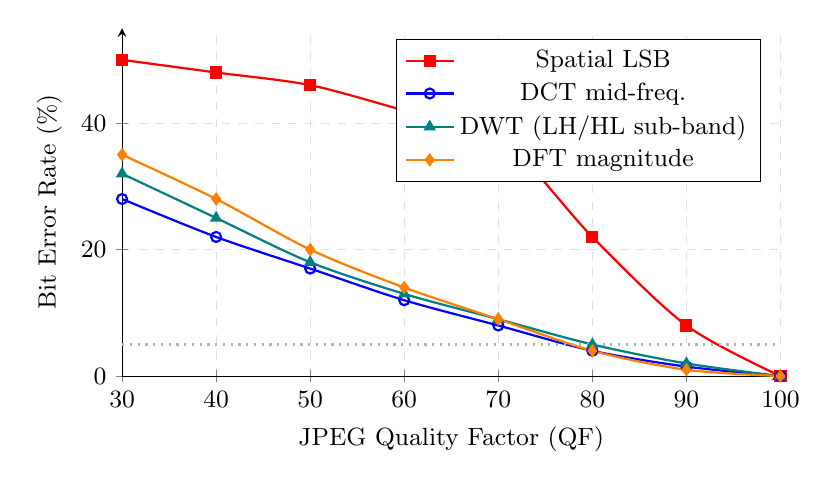
\begin{tikzpicture}
    \begin{axis}[
        width=0.82\textwidth, height=6.0cm,
        xlabel={JPEG Quality Factor (QF)},
        ylabel={Bit Error Rate (\%)},
        xmin=30, xmax=100,
        ymin=0,  ymax=55,
        xtick={30,40,50,60,70,80,90,100},
        legend pos=north east,
        legend style={font=\small},
        grid=major,
        grid style={dashed, gray!25},
        axis lines=left,
        tick label style={font=\small},
        label style={font=\small},
      ]
      % Spatial LSB (high freq) -- very sensitive to JPEG
      \addplot[thick, red, mark=square*, mark size=1.8pt, smooth] coordinates {
        (30,50)(40,48)(50,46)(60,42)(70,38)(80,22)(90,8)(100,0)
      };
      \addlegendentry{Spatial LSB}

      % DCT mid-freq -- moderate sensitivity
      \addplot[thick, blue, mark=o, mark size=1.8pt, smooth] coordinates {
        (30,28)(40,22)(50,17)(60,12)(70,8)(80,4)(90,1.5)(100,0)
      };
      \addlegendentry{DCT mid-freq.}

      % DWT HL/LH sub-bands
      \addplot[thick, teal, mark=triangle*, mark size=1.8pt, smooth] coordinates {
        (30,32)(40,25)(50,18)(60,13)(70,9)(80,5)(90,2)(100,0)
      };
      \addlegendentry{DWT (LH/HL sub-band)}

      % DFT magnitude (global -- somewhat more resilient than DCT)
      \addplot[thick, orange, mark=diamond*, mark size=1.8pt, smooth] coordinates {
        (30,35)(40,28)(50,20)(60,14)(70,9)(80,4)(90,1)(100,0)
      };
      \addlegendentry{DFT magnitude}

      % 5% BER threshold line
      \draw[dotted, thick, gray!60] (axis cs:30,5) -- (axis cs:100,5)
        node[right, font=\footnotesize, gray!70]{BER\,=\,5\%};
    \end{axis}
  \end{tikzpicture}
  \caption{Illustrative bit error rate (BER) as a function of JPEG quality factor for four
           embedding domains. Spatial LSB embedding is almost entirely destroyed below
           QF\,=\,90, while transform-domain methods show substantially better survival.
           The dotted line marks the $5\%$ BER threshold below which error correction coding
           can typically achieve full recovery. Curves are representative of trends reported
           in the literature \cite{cox2007digital, petitcolas1999information}.}
  \label{fig:jpeg_ber}
\end{figure}

\subsubsection{Additive Noise}

Additive noise arises from sensor imperfections during re-capture, analogue-to-digital conversion
errors, or deliberate noise injection by an adversary attempting to destroy hidden content. The
most common model is additive white Gaussian noise (AWGN) \cite{gonzalez2008digital}.

\paragraph{Formal degradation model.}
Let $I(x,y)$ denote the pixel intensity at location $(x,y)$ in the stego-image. Under AWGN,
the received signal is:

\begin{equation}
  \tilde{I}(x,y) = I(x,y) + \eta(x,y), \quad
  \eta(x,y) \sim \mathcal{N}(0,\, \sigma_n^2),
  \label{eq:awgn}
\end{equation}

where $\sigma_n^2$ is the noise variance and individual noise samples $\eta(x,y)$ are independent
and identically distributed. The signal-to-noise ratio of the stego-image under AWGN is:

\begin{equation}
  \mathrm{SNR} = 10 \log_{10} \!\left( \frac{\sigma_I^2}{\sigma_n^2} \right) \quad [\mathrm{dB}],
  \label{eq:snr}
\end{equation}

where $\sigma_I^2$ is the variance of the image signal. In the frequency domain, AWGN distributes
energy uniformly across all spatial frequencies, affecting both low- and high-frequency components.
This is qualitatively different from JPEG compression, which concentrates distortion in
high-frequency coefficients.

\paragraph{Impact on steganographic embedding.}
The effect of AWGN on an embedded steganographic signal of amplitude $\alpha$ depends on the
embedding domain. For spread-spectrum steganography, where each bit is spread across $N$
coefficients, the signal-to-noise ratio at the decoder is:

\begin{equation}
  \mathrm{SNR}_\text{dec} = \frac{\alpha^2 N}{\sigma_n^2},
  \label{eq:ss_snr}
\end{equation}

showing that the spreading gain $N$ provides a factor-of-$N$ improvement in noise robustness
relative to single-coefficient embedding \cite{marvel1999spread}. For DCT-domain embedding
at mid-frequencies, AWGN introduces errors only when $|\eta(x,y)|$ is large enough, after
transformation, to flip the decision boundary used in extraction.

Salt-and-pepper noise, an alternative model in which a fraction $p$ of pixels are set to
the maximum or minimum intensity value, is more destructive than AWGN per unit distortion
because it produces extreme outliers that cannot be corrected by averaging-based spreading.

\subsubsection{Filtering Attacks}

Filtering attacks apply a linear or non-linear convolution kernel to the image, altering the
spatial frequency content. Common instances include Gaussian blurring, median filtering, and
sharpening filters \cite{gonzalez2008digital}.

\paragraph{Formal degradation model.}
A linear low-pass filter applies a convolution:

\begin{equation}
  \tilde{I}(x,y) = I(x,y) * h(x,y)
    = \sum_{m} \sum_{n} I(x-m,\, y-n)\, h(m,n),
  \label{eq:lpf}
\end{equation}

where $h(x,y)$ is the filter kernel. The Gaussian blur kernel is:

\begin{equation}
  h_\sigma(x,y) = \frac{1}{2\pi\sigma^2}
    \exp\!\left(-\frac{x^2 + y^2}{2\sigma^2}\right),
  \label{eq:gaussian_kernel}
\end{equation}

with standard deviation $\sigma$ controlling the degree of blurring. In the frequency domain,
convolution becomes multiplication:

\begin{equation}
  \tilde{F}(u,v) = F(u,v) \cdot H(u,v),
  \label{eq:lpf_freq}
\end{equation}

where $H(u,v)$ is the Fourier transform of $h(x,y)$. For a Gaussian kernel, $H(u,v)$ is itself
a Gaussian centred at the origin, decaying to near zero at high frequencies. The attenuation
factor $H(u,v)$ for a Gaussian blur with $\sigma = 1.5$ already reduces mid-frequency components
by $30$--$60\%$, which is sufficient to destroy embeddings of moderate strength.

\paragraph{Impact on steganographic embedding.}
Low-pass filtering is particularly damaging to embeddings in high and mid-frequency DCT or
DWT coefficients, because the filter directly suppresses the spectral region used for embedding.
The fraction of the embedded signal that survives filtering is $H(u_0, v_0)$ at the embedding
frequency $(u_0, v_0)$. For a Gaussian blur with $\sigma = 2.0$, high-frequency DCT coefficients
($u+v \geq 10$) are attenuated by more than $90\%$, making unprotected high-frequency embedding
essentially non-survivable. Median filtering is additionally non-linear and cannot be described
by a single attenuation factor; it is particularly effective at destroying LSB-level spatial
embeddings.

% Figure suggestion (use a real image or pgfplots):
% Title: "Frequency-domain attenuation profiles of Gaussian blur at sigma=1, 1.5, 2.0,
%          showing progressive suppression of mid- and high-frequency DCT coefficients"
% Note: This is best illustrated with an actual 2D magnitude spectrum image side-by-side
%       with the filter's frequency response. Recommend generating with Python/Matplotlib
%       and including as a \includegraphics figure.

\subsubsection{Colour Space Conversion and Format Conversion}

Social media platforms frequently convert uploaded images between colour spaces (RGB to
YCbCr, RGB to greyscale) or between formats (JPEG to WebP, PNG to JPEG). Colour space
conversion alters the relationship between colour channels, potentially redistributing energy
between the luminance and chrominance components and disrupting embeddings that rely on
specific channel statistics \cite{cox2007digital}. Format conversion compounds this with
the quantisation effects of the target codec. A full print-scan cycle — printing a digital
image and re-capturing it with a camera — introduces all of the above simultaneously: blur,
noise, perspective distortion, and colour shift \cite{wengrowski2019light}.

% ----------------------------------------------------------
\subsection{Geometric Attacks}
\label{subsec:geometric_attacks}
% ----------------------------------------------------------

Geometric attacks alter the spatial arrangement of pixels rather than their intensity values.
They are qualitatively more destructive than signal processing attacks for most steganographic
systems because they introduce \emph{synchronisation loss}: the extractor can no longer locate
the embedding positions even when the embedded data itself is largely intact
\cite{ruanaidh1998rotation, cox2007digital}. Error correction coding cannot recover from
synchronisation loss because the codeword bits are read in the wrong order or from the wrong
positions, producing not random errors but structured misalignment that looks identical to
complete payload destruction.

\subsubsection{Cropping}

Cropping removes a contiguous rectangular region from the image, permanently deleting all
pixels — and all embedded data — within that region.

\paragraph{Formal degradation model.}
Let the original stego-image have dimensions $M \times N$. A crop operation retains a
sub-image starting at offset $(r_0, c_0)$ with dimensions $M' \times N'$, where
$M' < M$ or $N' < N$:

\begin{equation}
  \tilde{I}(x,y) = I(x + r_0,\, y + c_0), \quad
  0 \leq x < M',\; 0 \leq y < N'.
  \label{eq:crop}
\end{equation}

The fraction of the image area that is destroyed is:

\begin{equation}
  \rho_\text{crop} = 1 - \frac{M' \cdot N'}{M \cdot N}.
  \label{eq:crop_fraction}
\end{equation}

For a steganographic system that embeds $N_F$ fragments uniformly distributed across the image,
the expected number of fragments destroyed by a crop of fraction $\rho_\text{crop}$ is:

\begin{equation}
  \mathbb{E}[\text{fragments lost}] = N_F \cdot \rho_\text{crop},
  \label{eq:crop_fragments}
\end{equation}

assuming uniform spatial distribution of fragments. This is the key quantity that the proposed
self-recovering framework is designed to minimise by maximising spatial redundancy and
distribution of embedded fragments across non-contiguous image regions.

\paragraph{Synchronisation effect.}
Beyond the direct data loss of Equation~\eqref{eq:crop}, cropping destroys the coordinate
reference frame used during embedding. Block-based extractors (DCT, DWT) depend on knowing
the exact position of the top-left corner of the image to reconstruct the block grid. After
cropping, the origin shifts to $(r_0, c_0)$, misaligning every block by the crop offset. Even
a single-pixel crop offset causes every $8 \times 8$ DCT block to be misaligned, producing
a near-random BER. This effect is illustrated conceptually in
Figure~\ref{fig:crop_misalignment}.

\begin{figure}[htbp]
  \centering
  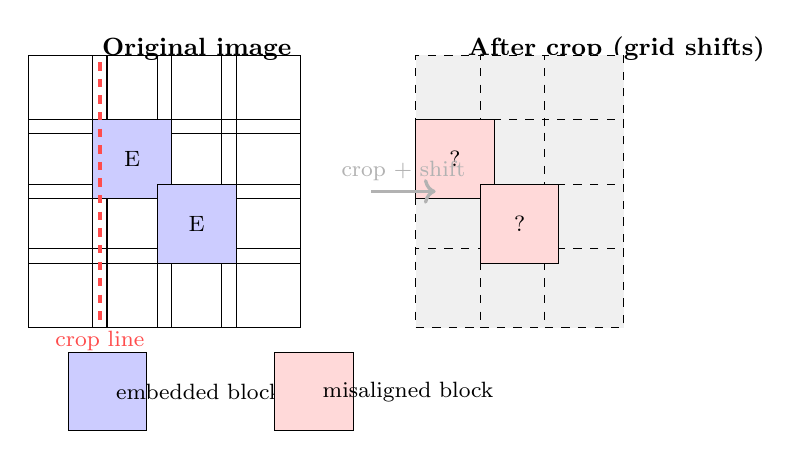
\begin{tikzpicture}[
      scale=0.82,
      block/.style={draw, minimum size=1.0cm, inner sep=0, font=\footnotesize},
      emb/.style={draw, minimum size=1.0cm, inner sep=0, fill=blue!20, font=\footnotesize},
      crop/.style={draw, minimum size=1.0cm, inner sep=0, fill=red!15, font=\footnotesize},
      miss/.style={draw, minimum size=1.0cm, inner sep=0, fill=gray!12,
                   font=\footnotesize, dashed},
    ]

    % ---- LEFT: original block grid ----
    \node[font=\small\bfseries] at (2.0, 0.7) {Original image};

    \foreach \col in {0,1,2,3} {
      \foreach \row in {0,-1,-2,-3} {
        \node[block] at (\col, \row) {};
      }
    }
    % Highlight two embedded blocks
    \node[emb] at (1,-1) {E};
    \node[emb] at (2,-2) {E};

    % Crop line (remove leftmost column)
    \draw[very thick, red!70, dashed]
      (0.5, 0.5) -- (0.5, -3.5)
      node[below, font=\footnotesize, red!70]{crop line};

    % ---- RIGHT: cropped image with shifted grid ----
    \node[font=\small\bfseries] at (8.5, 0.7) {After crop (grid shifts)};

    \foreach \col in {0,1,2} {
      \foreach \row in {0,-1,-2,-3} {
        \node[miss] at (6.0+\col, \row) {};
      }
    }
    % Embedded blocks now at wrong positions
    \node[crop] at (6.0, -1) {?};
    \node[crop] at (7.0, -2) {?};

    % Arrow
    \draw[->, very thick, gray!60] (4.7, -1.5) -- (5.7, -1.5)
      node[midway, above, font=\footnotesize]{crop + shift};

    % Legend
    \node[emb, right] at (0, -4.6) {};
    \node[font=\footnotesize, right] at (0.6, -4.6) {embedded block};
    \node[crop, right] at (3.2, -4.6) {};
    \node[font=\footnotesize, right] at (3.8, -4.6) {misaligned block};

  \end{tikzpicture}
  \caption{Effect of cropping on block-based DCT embedding. Removing even a single column
           of pixels shifts the entire block grid, causing the extractor to read coefficients
           from misaligned blocks. The embedded data (marked E) is now read from the wrong
           positions (marked ?), producing near-random extraction even though the data
           itself was not removed by the crop.}
  \label{fig:crop_misalignment}
\end{figure}

\subsubsection{Resizing and Resampling}

Resizing changes the spatial resolution of the image by either upsampling (increasing dimensions)
or downsampling (reducing dimensions) through pixel interpolation.

\paragraph{Formal degradation model.}
For a scaling factor $s$ (where $s < 1$ denotes downsampling and $s > 1$ upsampling), the
resized image is computed through a resampling filter:

\begin{equation}
  \tilde{I}(x,y) = \sum_{m} \sum_{n} I(m,n)\,
    k\!\left(\frac{x}{s} - m,\, \frac{y}{s} - n\right),
  \label{eq:resize}
\end{equation}

where $k(\cdot, \cdot)$ is an interpolation kernel. Common kernels are:

\begin{itemize}
  \item \textbf{Nearest-neighbour:} $k(t) = \mathbf{1}[|t| < 0.5]$ — fast but introduces
        blocking artefacts.
  \item \textbf{Bilinear:} $k(t) = \max(0, 1 - |t|)$ — linear interpolation between
        adjacent pixels; attenuates high-frequency content.
  \item \textbf{Bicubic:} a piecewise cubic kernel that provides better frequency
        preservation than bilinear but introduces slight ringing at edges \cite{gonzalez2008digital}.
\end{itemize}

\paragraph{Impact on steganographic embedding.}
Resampling has two effects. First, the interpolation kernel acts as a low-pass filter, attenuating
high-frequency components similarly to Gaussian blur. Second, and more critically, resampling at
a non-integer scale factor changes the pixel count, destroying the one-to-one correspondence
between embedding positions and extraction positions. For DCT-based embedding, downsampling
by a factor $s \neq 1$ shifts the $8 \times 8$ block boundaries to non-integer positions,
misaligning the extractor's grid. For spread-spectrum embedding, resampling alters the spatial
positions at which the pseudo-random spreading sequence is sampled, causing the correlation in
Equation~(2.16) to collapse \cite{marvel1999spread}.

\subsubsection{Rotation}

Rotation transforms the image by an angle $\theta$ about a centre point, resampling pixels from
their new positions.

\paragraph{Formal degradation model.}
The rotation transformation maps pixel coordinates $(x,y)$ to new coordinates $(x', y')$
according to:

\begin{equation}
  \begin{bmatrix} x' \\ y' \end{bmatrix}
  =
  \begin{bmatrix} \cos\theta & -\sin\theta \\ \sin\theta & \cos\theta \end{bmatrix}
  \begin{bmatrix} x - x_c \\ y - y_c \end{bmatrix}
  +
  \begin{bmatrix} x_c \\ y_c \end{bmatrix},
  \label{eq:rotation}
\end{equation}

where $(x_c, y_c)$ is the centre of rotation. Pixel values at non-integer coordinates
$(x', y')$ are obtained by interpolation. Rotation also typically introduces a band of
undefined pixels at the image boundary, which are either cropped or filled with a constant
value, further reducing the usable image area.

\paragraph{Impact on steganographic embedding.}
Even a small rotation of $\theta = 1°$ displaces pixels near the image boundary by several
pixels, making it impossible for a block-based extractor to locate its $8 \times 8$ grids.
For DFT-based steganography, the Fourier magnitude spectrum rotates by the same angle $\theta$
in the frequency domain, which preserves energy at the same radial frequency but shifts angular
position \cite{bracewell2000fourier}. This provides partial robustness: embeddings in
rotationally symmetric regions of the DFT spectrum (concentric rings) survive rotation, while
embeddings at specific angular positions do not. Log-polar DFT embedding achieves full
rotation-scale invariance but at significant capacity cost \cite{ruanaidh1998rotation}.

\subsubsection{Affine and Projective Transformations}

More general spatial transformations include affine mappings (combinations of rotation, scaling,
shearing, and translation) and projective (homographic) transformations, which arise in
print-scan scenarios where the camera is not perfectly parallel to the printed surface
\cite{kutter1999digital}. An affine transformation applies:

\begin{equation}
  \begin{bmatrix} x' \\ y' \end{bmatrix}
  =
  \mathbf{A}
  \begin{bmatrix} x \\ y \end{bmatrix}
  + \mathbf{t},
  \label{eq:affine}
\end{equation}

where $\mathbf{A}$ is a $2\times2$ matrix encoding rotation, scaling, and shear, and $\mathbf{t}$
is a translation vector. Projective transformations add perspective distortion, mapping straight
lines to straight lines but not preserving parallel lines or angles. Both classes of
transformation are highly destructive to all location-dependent steganographic methods and require
either invariant-domain embedding or template-based re-synchronisation for recovery
\cite{cox2007digital}.

% ----------------------------------------------------------
\subsection{Compound and Pipeline Attacks}
\label{subsec:compound_attacks}
% ----------------------------------------------------------

In practice, stego-images are rarely subjected to a single isolated attack. Real-world
distribution channels apply multiple operations sequentially, each building on the damage
introduced by the previous stage. This is the \emph{compound attack} or \emph{pipeline attack}
model, and it represents the most realistic and challenging threat scenario for any robust
steganographic system \cite{petitcolas1999information}.

\paragraph{Social media processing pipelines.}
Table~\ref{tab:platform_pipelines} summarises the documented processing pipelines applied to
uploaded images by major social media and messaging platforms. Each pipeline represents a
compound attack that a stego-image must survive if the steganographic channel is to function
through that platform.

\begin{table}[htbp]
  \centering
  \caption{Documented image processing operations applied by major social media and messaging
           platforms to uploaded images. The combination of these operations constitutes a
           compound attack on embedded steganographic payloads. QF: JPEG quality factor.
           Information compiled from \cite{jia2021mbrs, wengrowski2019light,
           petitcolas1999information}.}
  \label{tab:platform_pipelines}
  \renewcommand{\arraystretch}{1.3}
  \small
  \begin{tabular}{@{} l c c c c c @{}}
    \toprule
    \textbf{Platform} & \textbf{JPEG recompr.} & \textbf{Resize} &
    \textbf{Crop} & \textbf{Format conv.} & \textbf{Approx.\ QF} \\
    \midrule
    WhatsApp   & Yes & Yes (max 1600px) & Sometimes & JPEG      & 75--85 \\
    Instagram  & Yes & Yes (max 1080px) & Yes (square) & JPEG   & 70--80 \\
    Twitter/X  & Yes & Yes (max 4096px) & No         & JPEG/WebP & 85     \\
    Facebook   & Yes & Yes              & No         & JPEG      & 70--85 \\
    Telegram   & Yes & Sometimes        & No         & JPEG      & 90--95 \\
    \bottomrule
  \end{tabular}
\end{table}

\paragraph{Formal compound degradation model.}
A compound attack can be modelled as the sequential application of $K$ individual degradation
operators $\mathcal{D}_1, \mathcal{D}_2, \ldots, \mathcal{D}_K$:

\begin{equation}
  \tilde{I} = \mathcal{D}_K \circ \mathcal{D}_{K-1} \circ \cdots \circ \mathcal{D}_1 (I_s),
  \label{eq:compound}
\end{equation}

where $I_s$ is the stego-image and $\circ$ denotes function composition. The compound BER is
not simply the sum of the individual BERs; operators interact non-linearly. In particular,
geometric distortion followed by JPEG compression is far more destructive than either alone,
because the geometric operation shifts block boundaries and the subsequent JPEG re-compression
then operates on misaligned blocks, amplifying both synchronisation loss and quantisation error.

\paragraph{Empirical impact.}
Studies have shown that a WhatsApp-equivalent pipeline (resize to 1600px + JPEG QF\,=\,80)
reduces the BER recovery of a standard DCT mid-frequency embedding from approximately $8\%$
(JPEG alone) to over $35\%$, constituting near-total communication failure
\cite{jia2021mbrs, cox2007digital}. This motivates the need for a framework that addresses
compound attacks as a first-class design objective rather than evaluating individual attacks
in isolation.

% Figure: compound attack pipeline diagram
\begin{figure}[htbp]
  \centering
  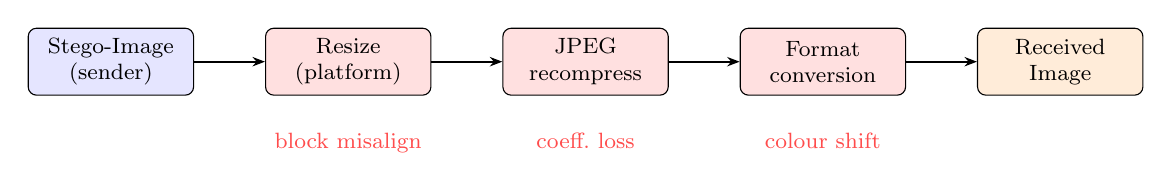
\begin{tikzpicture}[
      node distance = 0.5cm and 0.9cm,
      stage/.style = {draw, rounded corners=3pt, minimum width=2.1cm,
                      minimum height=0.85cm, align=center, font=\footnotesize,
                      fill=blue!10},
      attack/.style= {draw, rounded corners=3pt, minimum width=2.1cm,
                      minimum height=0.85cm, align=center, font=\footnotesize,
                      fill=red!12},
      result/.style= {draw, rounded corners=3pt, minimum width=2.1cm,
                      minimum height=0.85cm, align=center, font=\footnotesize,
                      fill=orange!15},
      arr/.style   = {-{Stealth[length=4.5pt]}, thick},
    ]

    \node[stage]  (stego)  {Stego-Image\\(sender)};
    \node[attack, right=of stego]  (resize) {Resize\\(platform)};
    \node[attack, right=of resize] (jpeg)   {JPEG\\recompress};
    \node[attack, right=of jpeg]   (format) {Format\\conversion};
    \node[result, right=of format] (recv)   {Received\\Image};

    \draw[arr] (stego)  -- (resize);
    \draw[arr] (resize) -- (jpeg);
    \draw[arr] (jpeg)   -- (format);
    \draw[arr] (format) -- (recv);

    % Damage annotations below
    \node[font=\footnotesize, red!70, below=0.35cm of resize]
      {block misalign};
    \node[font=\footnotesize, red!70, below=0.35cm of jpeg]
      {coeff.\ loss};
    \node[font=\footnotesize, red!70, below=0.35cm of format]
      {colour shift};

  \end{tikzpicture}
  \caption{A typical social media compound attack pipeline applied to a stego-image.
           Each stage introduces a distinct type of degradation: resizing causes block
           misalignment and acts as a low-pass filter; JPEG recompression introduces
           quantisation error in DCT coefficients; format conversion may introduce
           additional colour-space transformations. The cumulative effect is far more
           destructive than any single attack alone.}
  \label{fig:compound_pipeline}
\end{figure}

% ----------------------------------------------------------
\subsection{Steganalytic Attacks}
\label{subsec:attack_steganalysis}
% ----------------------------------------------------------

In addition to signal degradation and geometric distortion, steganographic systems face a
fundamentally different class of attack: \emph{steganalysis}, the statistical detection of
hidden communication. A steganalytic attack does not aim to destroy the hidden payload but to
determine whether one exists, thereby exposing the covert channel and potentially leading to
further scrutiny or interception \cite{Fridrich2012}.

\subsubsection{Statistical Detection Principles}

Cover images and stego-images differ in their statistical properties because the embedding
process necessarily alters the image signal. Statistical steganalysis exploits these differences
by computing feature vectors that capture deviations from the statistics of natural, unmodified
images \cite{Fridrich2012}. The Cartesian Calibration framework introduced by Fridrich and
Goljan \cite{fridrich2004attacks} models the statistical footprint of embedding as a deviation
from the ``natural image manifold'' and uses decompressed JPEG images as a calibration reference.

\paragraph{Classical steganalysis: targeted detectors.}
Early steganalytic attacks were algorithm-specific. The $\chi^2$ (chi-squared) attack
\cite{westfeld2001f5} exploits the symmetry in histogram pairs produced by LSB substitution:
embedding causes adjacent pixel value pairs $(2k, 2k+1)$ to equalise in frequency, a pattern
that is statistically impossible in natural images. The RS (Regular-Singular) analysis
\cite{provos2003hide} extends this to spatial neighbourhoods, achieving reliable detection
of LSB embedding at rates as low as $10\%$ bpp. Both attacks are algorithm-specific and fail
against other embedding methods.

\paragraph{Universal steganalysis.}
Modern steganalysis is algorithm-agnostic. The Rich Model (RM) framework of Fridrich and
Kodovský \cite{Fridrich2012} computes co-occurrence matrices of pixel residuals in multiple
directions and at multiple scales, constructing a feature vector of dimension $34\,671$.
Paired with an ensemble classifier, the Rich Model achieves near-perfect detection of
modern spatial-domain steganographic algorithms (WOW, HILL, S-UNIWARD) at embedding rates
of $0.4$\,bpp, and detection above chance at rates as low as $0.05$\,bpp. This effectively
closes the spatial domain for steganographic use at any non-trivial payload rate.

\paragraph{Deep learning steganalysis.}
As discussed in Section~\ref{subsec:dl_steganalysis}, deep neural network steganalysers
such as SRNet \cite{boroumand2019deep}, XuNet \cite{xu2016structural}, and Ye-Net
\cite{yedroudj2018yenet} extend universal steganalysis to a data-driven framework that
generalises across embedding algorithms and image sources, achieving detection performance
that exceeds the Rich Model on most benchmarks.

\subsubsection{Implications for Robustness-Oriented Design}

Steganalytic attacks impose a fundamental constraint on how robustness can be achieved.
As established in Section~2.3.7, increasing embedding strength improves signal-level
robustness but increases statistical detectability. This detectability--robustness trade-off
can be expressed formally: for a steganographic embedding that adds a signal of energy
$E_s$ to the cover image, both the PSNR (imperceptibility proxy) and the detectability
(as measured by the Area Under the ROC Curve, AUC, of a steganalytic classifier) are
monotonically related to $E_s$:

\begin{equation}
  \text{PSNR} \propto -\log E_s, \qquad
  \text{AUC} \propto f(E_s),
  \label{eq:detectability_tradeoff}
\end{equation}

where $f(\cdot)$ is a monotonically increasing function of $E_s$ \cite{Fridrich2012}.
Any design that increases $E_s$ to improve robustness therefore simultaneously increases
both detectability and distortion. This triple tension — robustness, imperceptibility,
undetectability — is the fundamental constraint that distinguishes robust steganographic
design from digital watermarking design.

This thesis treats steganalytic resistance as a secondary concern, explicitly noting that
the primary objective is payload survivability under degradation rather than undetectability.
However, the structural approach to robustness adopted in the proposed framework
(fragmentation, erasure coding, low-per-coefficient distortion) is inherently more
steganalysis-resistant than high-strength single-domain embedding, because the embedding
energy is distributed across a larger number of coefficients at lower individual distortion
per coefficient.

% ----------------------------------------------------------
\subsection{Unified Attack Summary and Implications for Framework Design}
\label{subsec:attack_summary}
% ----------------------------------------------------------

Table~\ref{tab:attack_summary} provides a comprehensive unified summary of all attack types
reviewed in this section, their formal degradation mechanisms, the steganographic failure
modes they introduce, and their relevance to the proposed self-recovering framework.

\begin{table}[htbp]
  \centering
  \caption{Unified summary of attack types, degradation mechanisms, failure modes, and
           implications for the proposed self-recovering framework. BER: Bit Error Rate;
           ECC: Error Correction Code; SS: Spread Spectrum; PRR: Partial Recovery Rate.}
  \label{tab:attack_summary}
  \renewcommand{\arraystretch}{1.35}
  \small
  \begin{tabular}{@{} p{2.1cm} p{2.5cm} p{2.4cm} p{2.0cm} p{3.4cm} @{}}
    \toprule
    \textbf{Attack} & \textbf{Degradation model} & \textbf{Failure mode} &
    \textbf{Survivable by} & \textbf{Framework implication} \\
    \midrule
    JPEG compression
      & Coefficient quantisation (Eq.~\ref{eq:jpeg_quant})
      & High BER in unstable coefficients
      & ECC, mid-freq.\ embedding
      & Embed in DCT mid-freq.; strength $> Q/2$ \\
    \midrule
    AWGN
      & Additive Gaussian (Eq.~\ref{eq:awgn})
      & Random bit flips
      & ECC, SS spreading
      & ECC at fragment level corrects noise errors \\
    \midrule
    Low-pass filtering
      & Convolution attenuation (Eq.~\ref{eq:lpf_freq})
      & Erasure of high-freq.\ embedding
      & Mid-freq.\ embedding
      & Avoid high-frequency subbands \\
    \midrule
    Cropping
      & Spatial erasure (Eq.~\ref{eq:crop}) + grid shift
      & Fragment loss + sync loss
      & Redundancy, fragmentation
      & Distributed fragments maximise PRR under crop \\
    \midrule
    Resizing
      & Interpolation (Eq.~\ref{eq:resize}) + scale shift
      & Block misalignment + signal attenuation
      & Invariant domains, multi-scale
      & Multi-scale redundant embedding reduces sensitivity \\
    \midrule
    Rotation
      & Coordinate transform (Eq.~\ref{eq:rotation}) + interpolation
      & Global synchronisation loss
      & Log-polar DFT, templates
      & DFT magnitude used for geometric-invariant copies \\
    \midrule
    Compound pipeline
      & Sequential composition (Eq.~\ref{eq:compound})
      & Cascaded signal + sync degradation
      & Structured redundancy only
      & Multi-domain distribution essential; no single domain sufficient \\
    \midrule
    Steganalysis
      & Statistical feature deviation
      & Channel exposure (not data loss)
      & Low distortion, structural embedding
      & Low per-coefficient distortion limits statistical footprint \\
    \bottomrule
  \end{tabular}
\end{table}

The most important observation from Table~\ref{tab:attack_summary} is the asymmetry between
signal processing attacks and geometric attacks in terms of their countermeasures. Signal
processing attacks introduce bit-level errors that can be corrected by ECC, provided that
synchronisation is maintained. Geometric attacks destroy synchronisation, making ECC
irrelevant because the bit order is lost. The proposed framework addresses this asymmetry
by maintaining synchronisation robustness through structured spatial distribution of fragments
(so that surviving fragments can be independently located) and multi-domain embedding (so that
the geometric invariance of DFT-domain copies provides fallback synchronisation when
block-based copies fail).

Compound attacks, which combine both classes of degradation, can only be addressed by a
system-level strategy that simultaneously tolerates signal-level errors and fragment-level
erasures. This is precisely the design philosophy of the self-recovering framework proposed
in Chapter~3: rather than optimising resistance to any single attack, the framework is
engineered to maintain a positive PRR — a non-zero fraction of recovered fragments — under
any compound attack that does not exceed the system's erasure budget.

\section{Discussion and Research Gap}

The literature reviewed in this chapter demonstrates significant progress in the field of image steganography, particularly in the development of transform-domain techniques and robustness-oriented embedding strategies. Methods based on DCT, DWT, and DFT have shown improved resistance to common signal processing operations compared to spatial-domain approaches, especially under mild compression and noise conditions \cite{cox2007digital}. However, despite these advancements, existing techniques continue to exhibit fundamental limitations when deployed in realistic and uncontrolled digital environments.

A primary limitation of conventional steganographic systems lies in their vulnerability to compound attacks. While many methods are evaluated against individual distortions such as JPEG compression or additive noise, real-world scenarios frequently involve sequential or combined operations, including compression followed by resizing or cropping. Under such conditions, robustness rapidly degrades, revealing the inadequacy of approaches that focus on isolated attack resistance rather than holistic survivability.

Robustness-oriented techniques, including the use of error correction codes and controlled redundancy, have been widely adopted to mitigate bit-level corruption caused by signal processing attacks \cite{cox2007digital}. Although these methods can significantly reduce extraction errors under noise and compression, they fail to address the synchronization problem introduced by geometric transformations. Cropping, resizing, and rotation disrupt spatial alignment and block correspondence, rendering the embedded data inaccessible even when it remains partially present within the image \cite{Piva2002}. This desynchronization represents a fundamental challenge that cannot be resolved through redundancy alone.

Several synchronization-aware solutions have been proposed, such as invariant-domain embedding, feature-based alignment, and template-based synchronization markers \cite{ruanaidh1998rotation}. While these approaches improve resistance to limited geometric distortions, they often introduce substantial overhead, reduce embedding capacity, or remain vulnerable to severe or compound transformations. Consequently, existing systems remain heavily dependent on accurate localization of embedding positions, making them fragile in the presence of uncontrolled spatial modifications.

Another critical observation from the literature is the conceptual overlap between robust steganography and digital watermarking. Although both domains employ similar robustness-enhancing techniques, their objectives differ fundamentally. Watermarking prioritizes persistent detectability for ownership verification, whereas steganography requires covert communication with minimal statistical detectability \cite{cox2007digital,provos2003hide}. Many robustness-driven methods implicitly shift toward watermarking paradigms, weakening the steganographic requirement of secrecy while still failing to guarantee data recovery under severe distortions.

Furthermore, intentional detection attacks in the form of steganalysis present an additional challenge. Modern steganalysis techniques exploit statistical anomalies and learned feature representations to identify hidden communication \cite{Fridrich2012}. The literature indicates a clear trade-off between robustness and undetectability, as strategies that enhance survivability—such as stronger embedding or redundancy—may increase statistical detectability. Although steganalysis resistance is not the primary focus of this thesis, its existence highlights the need for carefully balanced design choices in robust steganographic systems.

Recent deep learning-based steganographic approaches attempt to address some of these challenges through data-driven optimization \cite{hayes2017,ye2017}. While these methods demonstrate promising performance under trained conditions, their reliance on large datasets, lack of interpretability, and sensitivity to unseen or compound attacks limit their applicability for controlled robustness analysis. Moreover, learned models provide limited insight into synchronization behavior and payload survivability under geometric distortions, which remain central challenges in robust steganography.

Collectively, these observations reveal a critical research gap in existing work. Current steganographic systems predominantly focus on protecting embedding locations and coefficients rather than ensuring the survivability of the hidden payload itself. Robustness is often evaluated in terms of local signal preservation, while the ability to recover meaningful information under partial data loss and desynchronization remains largely unexplored.

Figure 2.X: Comparison between embedding-centric robustness and payload-oriented survivability

Figure 2.Y: Impact of signal processing and geometric attacks on synchronization and data recovery

This thesis addresses this gap by shifting the design focus from embedding-centric robustness to payload-oriented survivability. Instead of assuming perfect synchronization or complete data preservation, the proposed framework emphasizes structured message fragmentation, controlled redundancy, and multi-domain distribution to enable partial recovery under severe and compound image degradation. By tolerating data loss and synchronization imperfections, the framework aims to achieve reliable covert communication in hostile and uncontrolled digital environments.


% =========================

% ============================================================
\section{Recent Advances in Deep Learning-Based Steganography}
\label{sec:dl_steganography}
% ============================================================

The preceding sections have reviewed the classical foundations of robust image steganography,
covering spatial-domain techniques, frequency-domain transforms (DCT, DWT, DFT), and
robustness-oriented design strategies developed primarily between the late 1990s and the mid-2010s.
Since 2018, however, the field has undergone a dramatic transformation driven by the application
of deep learning. Convolutional neural networks (CNNs), generative adversarial networks (GANs),
and attention-based architectures have been adapted to the steganographic task, promising
simultaneous optimisation of imperceptibility, payload capacity, and robustness in ways that
classical hand-crafted methods cannot easily achieve.

This section surveys the most influential deep learning-based steganographic systems published
between 2018 and 2024, with particular attention to their robustness properties and the extent to
which they address the payload-survivability problem that motivates the present work. The section
concludes with a critical assessment of the limitations of data-driven approaches and an explicit
justification for the classical model-driven framework adopted in this thesis.

% ----------------------------------------------------------
\subsection{The Shift Toward End-to-End Learned Steganography}
\label{subsec:dl_shift}
% ----------------------------------------------------------

Classical steganographic systems are hand-engineered: the designer chooses a transform domain,
selects embedding positions, fixes an embedding rule, and derives extraction analytically from the
same rule. Every component is transparent and interpretable. The limitation is that design
decisions are made independently and are therefore individually sub-optimal; in particular,
embedding positions and strengths are chosen without direct knowledge of how a specific attack
will affect the received signal.

Deep learning approaches to steganography replace this modular pipeline with a single
differentiable system trained end-to-end on a large corpus of natural images
\cite{zhu2018hidden, baluja2017hiding}. In the typical architecture, an \emph{encoder} network
$E_\theta$ maps a cover image $C$ and a secret message $M$ to a stego-image $S$:
%
\begin{equation}
  S = E_\theta(C,\, M),
  \label{eq:encoder}
\end{equation}
%
while a \emph{decoder} network $D_\phi$ recovers the message from a (possibly degraded) received
signal $\tilde{S}$:
%
\begin{equation}
  \hat{M} = D_\phi(\tilde{S}).
  \label{eq:decoder}
\end{equation}
%
Training minimises a composite loss:
%
\begin{equation}
  \mathcal{L} = \lambda_1\,\mathcal{L}_{\text{img}}(C,S)
              + \lambda_2\,\mathcal{L}_{\text{msg}}(M,\hat{M})
              + \lambda_3\,\mathcal{L}_{\text{adv}},
  \label{eq:loss}
\end{equation}
%
where $\mathcal{L}_{\text{img}}$ penalises perceptible distortion between the cover and
stego-images, $\mathcal{L}_{\text{msg}}$ penalises errors in the recovered message, and
$\mathcal{L}_{\text{adv}}$ is an optional adversarial term from a discriminator trained to
detect the stego-image \cite{hayes2017}. The weights $\lambda_1, \lambda_2, \lambda_3$
control the balance between the three steganographic objectives. The key advantage over classical
methods is that gradient back-propagation allows the encoder and decoder to co-adapt: the encoder
learns to embed information in regions that the decoder can reliably read, even after passing
through a differentiable noise model that simulates real-world attacks during training.

% Figure: generic encoder-decoder-noise architecture
\begin{figure}[htbp]
  \centering
  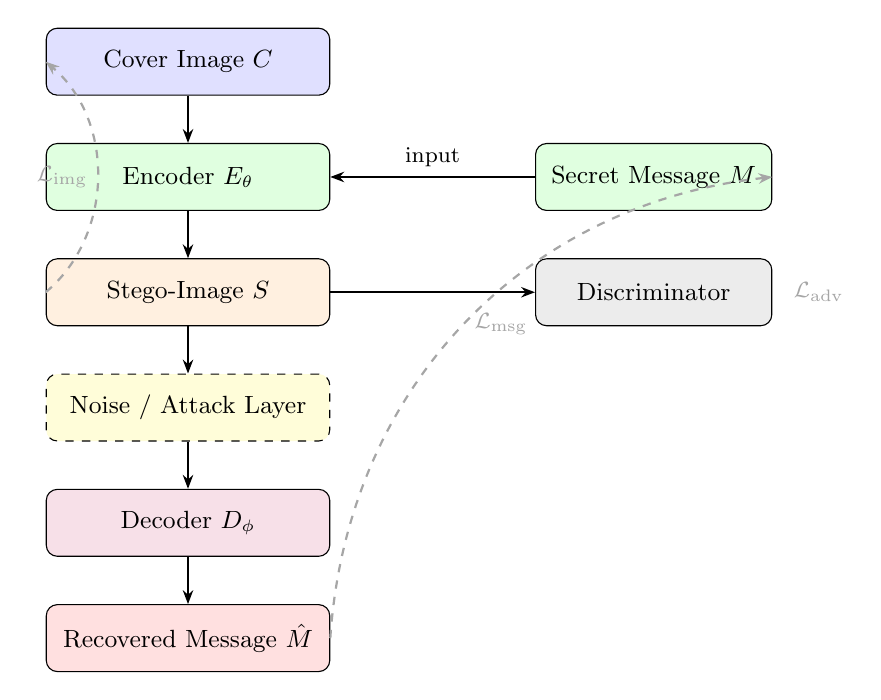
\begin{tikzpicture}[
      node distance = 0.6cm and 2.2cm,
      box/.style  = {draw, rounded corners=4pt, minimum width=3.6cm,
                     minimum height=0.85cm, align=center, font=\small},
      noisy/.style= {draw, dashed, rounded corners=4pt, minimum width=3.6cm,
                     minimum height=0.85cm, align=center, font=\small, fill=yellow!15},
      side/.style = {draw, rounded corners=4pt, minimum width=3.0cm,
                     minimum height=0.85cm, align=center, font=\small},
      arr/.style  = {-{Stealth[length=5pt]}, thick},
      darr/.style = {-{Stealth[length=5pt]}, thick, dashed, gray!70}
    ]

    % ---- LEFT COLUMN: main forward pipeline (top to bottom) ----
    \node[box, fill=blue!12]   (cover)  {Cover Image $C$};
    \node[box, fill=green!12,  below=of cover]  (enc)   {Encoder $E_\theta$};
    \node[box, fill=orange!12, below=of enc]    (stego) {Stego-Image $S$};
    \node[noisy,               below=of stego]  (noise) {Noise / Attack Layer};
    \node[box, fill=purple!12, below=of noise]  (dec)   {Decoder $D_\phi$};
    \node[box, fill=red!12,    below=of dec]    (msg)   {Recovered Message $\hat{M}$};

    % ---- RIGHT COLUMN: training-side components ----
    \node[side, fill=green!12, right=2.6cm of enc]    (secret) {Secret Message $M$};
    \node[side, fill=gray!15,  right=2.6cm of stego]  (disc)   {Discriminator};

    % ---- Main pipeline arrows ----
    \draw[arr] (cover) -- (enc);
    \draw[arr] (enc)   -- (stego);
    \draw[arr] (stego) -- (noise);
    \draw[arr] (noise) -- (dec);
    \draw[arr] (dec)   -- (msg);

    % ---- Side input arrows ----
    \draw[arr] (secret) -- (enc)
        node[midway, above, font=\footnotesize]{input};
    \draw[arr] (stego)  -- (disc);

    % ---- Loss feedback arrows (dashed) ----
    % L_img: from cover down to stego level, then right
    \draw[darr] (stego.west)
        to[bend right=50]
        node[left, font=\footnotesize]{$\mathcal{L}_\text{img}$}
        (cover.west);

    % L_msg: from recovered message back up to secret
    \draw[darr] (msg.east)
        to[bend left=40]
        node[right, font=\footnotesize]{$\mathcal{L}_\text{msg}$}
        (secret.east);

    % L_adv label next to discriminator
    \node[font=\footnotesize, gray!70, right=0.15cm of disc] {$\mathcal{L}_\text{adv}$};

  \end{tikzpicture}
  \caption{Generic encoder--decoder architecture for deep steganography.
           The main pipeline (left column) flows top-to-bottom: the encoder
           $E_\theta$ embeds the secret message into a cover image, the noise
           layer simulates attacks during training, and the decoder $D_\phi$
           recovers the message. Training-side components (right column) provide
           the message loss $\mathcal{L}_\text{msg}$ and an adversarial
           discriminator loss $\mathcal{L}_\text{adv}$; the image loss
           $\mathcal{L}_\text{img}$ (dashed, left) penalises visible distortion
           between cover and stego-image.}
  \label{fig:encoder_decoder}
\end{figure}

% ----------------------------------------------------------
\subsection{HiDDeN: The Foundational Framework (2018)}
\label{subsec:hidden}
% ----------------------------------------------------------

The most influential early work in the deep steganography paradigm is HiDDeN
(\textit{Hiding Data with Deep Networks}) by Zhu~et~al.\ \cite{zhu2018hidden}, presented at ECCV
2018. HiDDeN introduced three key ideas that have since become standard in the field.

\paragraph{Architecture.}
HiDDeN employs fully convolutional encoder and decoder networks.  The encoder is a
$7$-layer CNN that takes the cover image and a binary secret message (replicated to match the
spatial dimensions of the image) and outputs a stego-image of the same resolution. The decoder
is an independent CNN that maps a received stego-image directly back to the binary message
without any positional information. Neither network uses explicit transform-domain computation;
the optimal embedding strategy is learned implicitly from data.

\paragraph{Differentiable noise layer.}
The central contribution of HiDDeN is the insertion of a differentiable noise layer between the
encoder and decoder during training. The noise layer is a parametric module that randomly applies
one or more of the following operations to the stego-image before it reaches the decoder: JPEG
compression (approximated by a differentiable relaxation), Gaussian noise addition, dropout (random
pixel zeroing, simulating cropping of small regions), and Gaussian blurring. Because all operations
are differentiable with respect to their inputs, gradients flow back through the noise layer to the
encoder during training, causing the encoder to learn embeddings that are specifically resistant to
the attacks it will encounter at inference time. This is a fundamental architectural insight that
distinguishes HiDDeN from classical ECC-based approaches: rather than correcting errors after they
occur, the system learns to avoid them at the point of embedding.

\paragraph{Adversarial imperceptibility.}
HiDDeN adds a discriminator network trained to classify images as cover or stego. The
discriminator loss is added to the training objective of the encoder, creating a min-max game that
encourages the encoder to produce stego-images that are statistically indistinguishable from natural
photographs. This is conceptually similar to the GAN training paradigm introduced by
Goodfellow~et~al.\ \cite{goodfellow2014generative}, applied to the steganographic context.

\paragraph{Reported performance.}
On the COCO dataset, HiDDeN achieves a PSNR above $33$\,dB for $30$-bit payloads under JPEG
compression and Gaussian noise, with bit error rates below $1\%$, significantly outperforming
the classical F5 algorithm \cite{westfeld2001f5} under equivalent attack conditions.

The limitations of HiDDeN, however, are equally significant. The noise layer must be fixed before
training; if the deployed system encounters attacks not represented in the noise layer (e.g.\
spatial warping, format conversion chains, or aggressive cropping of large image fractions), the
encoder has learned no strategy to resist them. This is the distribution-shift problem that recurs
throughout deep steganography.

% ----------------------------------------------------------
\subsection{SteganoGAN: High-Capacity GAN-Based Steganography (2019)}
\label{subsec:steganogan}
% ----------------------------------------------------------

Zhang~et~al.\ \cite{zhang2019steganogan} introduced SteganoGAN in 2019, extending the
HiDDeN framework with a focus on maximising embedding capacity while preserving perceptual
quality. SteganoGAN proposes three encoder architectures of increasing depth — \emph{basic},
\emph{residual}, and \emph{dense} — corresponding to different trade-offs between capacity and
visual quality. The dense encoder, inspired by DenseNet \cite{huang2017densely}, concatenates
feature maps from all preceding layers, allowing the network to leverage both low-level texture
features and high-level semantic features when deciding where and how strongly to embed each
payload bit.

\paragraph{Key contributions.}
The primary innovation in SteganoGAN is a rigorous treatment of the capacity--quality trade-off.
The authors report that their dense encoder achieves capacities of up to $4.4$\,bpp (bits per
pixel) at a PSNR of $30.5$\,dB, compared to approximately $1.5$\,bpp for HiDDeN at equivalent
quality. The critical observation for the present work, however, is that SteganoGAN \emph{does
not include a noise layer}: training is performed under ideal (no-attack) conditions. The
resulting stego-images are therefore visually excellent but highly fragile. Under JPEG compression
at quality factor 70, the bit error rate of a SteganoGAN-trained decoder rises above $40\%$, which
constitutes complete communication failure. This confirms that capacity-oriented deep models
without explicit robustness training are unsuitable for uncontrolled transmission channels.

\paragraph{Relevance to this thesis.}
SteganoGAN illustrates a general principle that pervades both classical and deep steganography: in
the absence of specific robustness mechanisms, higher capacity invariably leads to lower
survivability. The dense architectures of SteganoGAN produce visually imperceptible embeddings but
exploit fragile, high-frequency image regions for extra capacity, exactly the regions that are
discarded by lossy compression.

% ----------------------------------------------------------
\subsection{ReDMark: Robustness-First Deep Steganography (2021)}
\label{subsec:redmark}
% ----------------------------------------------------------

Recognising the limitations of capacity-first approaches, Das~et~al.\ \cite{das2021redmark}
introduced ReDMark (\textit{Re-distributing the Weights for Robustness Deep Steganographic
Marking}) in 2021, the first deep steganographic system explicitly designed around the
robustness objective as the primary design constraint.

\paragraph{Architecture and training.}
ReDMark employs a U-Net-style encoder \cite{ronneberger2015unet} with skip connections that
propagate spatial information from the cover image directly to the deeper layers of the embedding
network. This architectural choice is motivated by the observation that skip connections encourage
the encoder to modulate existing image structures rather than superimpose an independent embedding
signal, resulting in stego-images that survive compression better because the embedding is
``anchored'' to stable image features that compression itself preserves.

The training pipeline of ReDMark incorporates a differentiable JPEG approximation module
\cite{shin2017jpeg} that accurately models the quantisation artifacts produced by the standard
JPEG codec. Additionally, a spatial transformer network (STN) \cite{jaderberg2015spatial} is
inserted in the noise layer to simulate mild geometric transformations (rotation by up to $5°$
and scaling by up to $20\%$), allowing the decoder to learn a degree of geometric invariance.

\paragraph{Loss function and weight redistribution.}
The distinctive contribution of ReDMark is a dynamic loss-weight redistribution scheme.
During training, the weights $\lambda_1$ and $\lambda_2$ in Equation~\eqref{eq:loss} are
adjusted adaptively based on the current attack intensity estimated from a running average of
recent BER values. When the bit error rate under the noise layer is high, the training procedure
temporarily increases $\lambda_2$ (message fidelity) relative to $\lambda_1$ (image quality),
forcing the encoder to prioritise robustness over imperceptibility until performance stabilises.
This curriculum-style approach avoids the common failure mode in which the encoder converges to
an imperceptible but fragile embedding from which it cannot escape by small gradient steps.

\paragraph{Reported performance.}
ReDMark achieves a PSNR of $36.2$\,dB at $30$-bit payload with a BER of $1.4\%$ after JPEG
compression at quality factor 50, and remains below $5\%$ BER under moderate rotation ($\leq 3°$)
and scaling ($\leq 10\%$). These results represent a meaningful advance over HiDDeN and
SteganoGAN under the same attack conditions.

\paragraph{Limitations.}
Despite these improvements, ReDMark retains the fundamental distribution-shift vulnerability.
Its resistance to geometric attacks extends only to the mild transformations simulated during
training. Under large-scale cropping (removal of $>30\%$ of image content) or compound attacks
combining JPEG compression with significant resizing (e.g.\ the pipeline applied by Twitter and
WhatsApp), the BER rises sharply. Furthermore, ReDMark, like all decoder-only deep methods,
provides no mechanism for partial recovery: if the bit error rate exceeds the decoder's
correction capability, the output is unintelligible, and no information about which fragments
of the payload survived is available.

% ----------------------------------------------------------
\subsection{Hiding Images in Images: High-Capacity Deep Concealment}
\label{subsec:hiding_images}
% ----------------------------------------------------------

A parallel line of deep steganographic research is concerned not with hiding binary messages
but with concealing entire images within other images. Baluja \cite{baluja2017hiding} introduced
a CNN-based framework for hiding a secret image within a cover image of the same dimensions,
using a ``preparation'' network to transform the secret image into a residual-ready representation
before the hiding network embeds it into the cover. The reveal network then reconstructs the
secret image from the stego-image with high fidelity (PSNR above $30$\,dB for both the
stego-image and the revealed secret).

\noindent
Lu~et~al.\ \cite{lu2021large} extended this paradigm to \emph{large-capacity} image hiding,
proposing an invertible neural network (INN) architecture \cite{dinh2017density} that is
mathematically reversible: the same network parameters are used for both embedding and
extraction by exploiting the invertibility of normalising flows. This guarantees that in the
absence of any attack, perfect recovery is possible. Under compression attacks, however, the
invertibility is broken, and recovery degrades.

While the image-in-image paradigm is not directly applicable to the binary message concealment
task of this thesis, it illustrates the general capacity of deep architectures to learn complex,
content-adaptive embeddings that far exceed the capacity of classical transform-domain methods.

% ----------------------------------------------------------
\subsection{Robust Deep Steganography Against Social Network Processing}
\label{subsec:social_network}
% ----------------------------------------------------------

A practically important research direction targets the specific degradation pipelines applied by
social media platforms (Instagram, Twitter, WhatsApp, Facebook), which combine JPEG recompression,
resolution rescaling, colour-space conversion, and sometimes format conversion (e.g.\ JPEG to
WebP). These operations collectively remove a large fraction of the information embedded by
conventional and naive deep steganographic methods.

Wengrowski and Dana \cite{wengrowski2019light} proposed a differentiable model of the photographic
process (capture, print, display, and re-capture), enabling a neural steganographic system to
survive the full print-scan loop. Their system produces cover-looking images that can be
photographed with a mobile camera and decoded with the neural decoder, surviving both compression
and optical blur.

Jia~et~al.\ \cite{jia2021mbrs} introduced MBRS (\textit{Mini-Batch of Real and Simulated JPEG
Compression}), in which each training mini-batch contains stego-images processed by both a
differentiable JPEG simulation and a \emph{real} JPEG codec. Including real JPEG artifacts in the
training data closes the gap between the differentiable approximation and the actual codec behaviour,
yielding substantially lower BER under real-world JPEG compression compared to methods trained on
differentiable approximations alone. MBRS achieves $0.9\%$ BER at $30$-bit payload under JPEG
quality factor 50 and $1.3\%$ under quality factor 30, with a stego-image PSNR of $38.1$\,dB.

% ----------------------------------------------------------
\subsection{Attention Mechanisms and Semantic-Aware Embedding}
\label{subsec:attention}
% ----------------------------------------------------------

Transformer-based architectures and spatial attention mechanisms have been applied to
steganography to improve both imperceptibility and robustness by enabling the network to
focus embedding on semantically stable image regions.

Luo~et~al.\ \cite{luo2020distortion} proposed a \emph{distortion-agnostic} deep hiding network
that uses a channel-spatial attention module to estimate the local imperceptibility budget at each
pixel, concentrating embedding in texture-rich regions (similar to the JND-based adaptive
embedding discussed in Section~2.3.4) while learning the content of those regions from data
rather than from hand-crafted JND models. The attention weights are updated jointly with the
encoder and decoder weights during training, allowing the system to adapt its embedding map
to the statistics of natural images.

Zhang~et~al.\ \cite{zhang2020udh} introduced UDH (\textit{Universal Deep Hiding}), a framework
in which the encoder learns a single, universal embedding pattern that is content-independent,
i.e.\ the same residual signal is added to any cover image regardless of its content. While
this reduces capacity compared to content-adaptive methods, it makes the embedding pattern
universal and more predictable under attacks, which simplifies decoder design.

% ----------------------------------------------------------
\subsection{Hybrid Transform-Network Approaches}
\label{subsec:hybrid}
% ----------------------------------------------------------

A natural development in the field is the combination of classical frequency-domain transforms
with learned components, seeking to obtain the theoretical guarantees and interpretability of
transform-domain methods alongside the adaptivity of data-driven approaches.

Ahmadi~et~al.\ \cite{ahmadi2020redmark} proposed a framework in which the encoder operates
in the DCT domain: DCT coefficients are first extracted from the cover image, and the neural
network learns to modify a selected subset of mid-frequency coefficients as a function of both
the cover content and the secret message. The extraction network inverts this process in the
DCT domain. This hybrid approach inherits the JPEG-robustness advantage of DCT embedding and
the adaptivity advantage of learned coefficient selection, achieving PSNR of $40.1$\,dB and
BER of $2.1\%$ under JPEG quality factor 70.

Fernandez~et~al.\ \cite{fernandez2023stable} explored the integration of steganography with
latent diffusion models, embedding messages in the latent space of a pre-trained image
generator. This approach exploits the perceptual quality of modern generative models to produce
stego-images that are virtually indistinguishable from natural photographs, at the cost of
requiring a generative model at inference time and being restricted to the image manifold of
the training data.

% ----------------------------------------------------------
\subsection{Deep Learning Steganalysis and Its Impact on Robust Design}
\label{subsec:dl_steganalysis}
% ----------------------------------------------------------

The same deep learning revolution that has advanced steganographic embedding has also produced
substantially more powerful steganalytic detectors. The SRNet architecture of Boroumand~et~al.\
\cite{boroumand2019deep} achieves near-perfect detection of several state-of-the-art spatial-domain
and DCT-domain steganographic algorithms using a single, unified deep network, without any
algorithm-specific feature engineering. More recently, the XuNet \cite{xu2016structural} and
Ye-Net \cite{yedroudj2018yenet} architectures have demonstrated that deep classifiers trained on
the StegoAppDB dataset generalise across embedding algorithms, significantly raising the bar for
undetectability.

These developments have important implications for the design of robust steganographic systems.
Because deep steganalysis is both universal (algorithm-agnostic) and sensitive (detecting payloads
at embedding rates well below $0.1$\,bpp in spatial-domain methods), any strategy that increases
embedding strength for the sake of robustness automatically increases the statistical footprint
detectable by a deep steganalyser. This confirms and deepens the detectability--robustness
trade-off discussed in Section~2.3.7, and reinforces the motivation for structural robustness
approaches (fragmentation, erasure coding, domain diversity) that can maintain a low per-pixel
distortion while still enabling payload survivability.

% ----------------------------------------------------------
\subsection{Summary Table and Comparative Analysis}
\label{subsec:dl_summary_table}
% ----------------------------------------------------------

Table~\ref{tab:dl_comparison} summarises the deep learning-based methods reviewed in this
section alongside the classical methods from Section~2.3, providing a unified comparative view.

\begin{table}[htbp]
  \centering
  \caption{Comparative summary of deep learning-based steganographic methods (2018--2024)
           alongside selected classical baselines. Performance figures are indicative only
           and refer to $30$-bit payloads on natural image datasets under JPEG QF\,=\,70 unless
           otherwise noted. BER: Bit Error Rate; PSNR: Peak Signal-to-Noise Ratio.}
  \label{tab:dl_comparison}
  \small
  \renewcommand{\arraystretch}{1.3}
  \begin{tabular}{@{} l l c c c c @{}}
    \toprule
    \textbf{Method} & \textbf{Year} & \textbf{PSNR (dB)} & \textbf{BER (\%)} &
    \textbf{Geo.\ Rob.} & \textbf{Partial Rec.} \\
    \midrule
    DCT mid-freq.\ (classical) & ---  & $\approx\!38$ & $\approx\!15$ & Poor & No \\
    LSB spatial (classical)    & ---  & $\approx\!51$ & $\approx\!50$ & Poor & No \\
    \midrule
    HiDDeN \cite{zhu2018hidden}         & 2018 & 33.1 & 0.5  & Limited & No \\
    SteganoGAN \cite{zhang2019steganogan}& 2019 & 30.5 & 40+ (JPEG) & None & No \\
    ReDMark \cite{das2021redmark}        & 2021 & 36.2 & 1.4  & Limited & No \\
    MBRS \cite{jia2021mbrs}             & 2021 & 38.1 & 0.9  & Limited & No \\
    UDH \cite{zhang2020udh}             & 2020 & 34.8 & 2.2  & Limited & No \\
    DCT-hybrid \cite{ahmadi2020redmark} & 2020 & 40.1 & 2.1  & Limited & No \\
    \midrule
    \textbf{Proposed framework}         & 2025 & ---  & ---  & Designed & \textbf{Yes} \\
    \bottomrule
  \end{tabular}
\end{table}

The critical observation from Table~\ref{tab:dl_comparison} is consistent with the finding of
Table~2.1 in Section~2.3.9: no existing deep learning system, including the most recent
state-of-the-art methods, provides mechanisms for \emph{partial recovery} of the hidden payload
when large portions of the stego-image are destroyed. All deep decoders operate in a binary
succeed-or-fail mode: they either reconstruct the entire message or produce unintelligible output.
This is a fundamental architectural limitation of the encoder-decoder paradigm, not a parameter
that can be tuned.

% ----------------------------------------------------------
\subsection{Why This Thesis Adopts a Classical Framework}
\label{subsec:justification}
% ----------------------------------------------------------

The review in this section makes clear that deep learning-based steganography represents the
current state of the art in terms of raw imperceptibility and robustness to trained attacks.
Nevertheless, the present thesis adopts a classical, model-driven framework for several reasons
that are directly related to the specific research objectives defined in Chapter~1.

\paragraph{Partial recovery as a first-class design objective.}
The primary objective of this thesis is to design a system that can recover \emph{usable
information} from a partially destroyed stego-image, rather than a system that achieves the
lowest BER under a fixed set of trained attacks. As established above, no existing deep learning
framework provides partial recovery capabilities; the encoder-decoder paradigm produces a
holistic encoding of the entire payload, and the decoder requires the full encoded signal to
function. Classical fragmentation and erasure-coding strategies (Section~2.3.5) are directly
applicable to the partial-recovery objective in a way that is not yet achievable with deep
architectures.

\paragraph{Robustness to \emph{unseen} compound attacks.}
Deep steganographic systems are robust only to the attacks represented in the training noise layer.
Social media platforms change their processing pipelines frequently, and different platforms apply
different combinations of compression quality, resize ratios, and format conversions. A classical
system whose robustness derives from structural properties of the payload (redundancy, distributed
embedding, erasure coding) is robust by construction to any attack that does not exceed its
erasure budget, regardless of whether that specific attack was anticipated during design. This
generalisation property is especially important for deployment in uncontrolled environments.

\paragraph{Interpretability and analytical robustness guarantees.}
A classical steganographic framework admits formal analysis: given a specified attack model, one
can compute (or bound) the probability that a given fragment survives, and hence the probability
that the payload is recovered. Deep learning systems provide no such guarantees; their robustness
is empirical and may degrade in ways that are difficult to predict. For applications in which
reliability is a hard requirement, interpretability and analytical tractability are significant
advantages.

\paragraph{Computational accessibility.}
Training a competitive deep steganographic system requires large-scale image datasets (typically
tens of thousands of images) and GPU-accelerated computing infrastructure for extended training
runs (often 24--100 hours). The classical framework proposed in this thesis is fully implementable
on standard hardware without any training phase, making it accessible in resource-constrained
environments.

\paragraph{Modularity and domain expertise.}
The classical framework allows individual components (the ECC scheme, the fragmentation strategy,
the embedding domain, the embedding strength) to be adjusted independently based on the properties
of the specific deployment environment. In a deep system, these design choices are entangled within
the network weights and cannot be modified without retraining. This modularity is particularly
valuable when the attack model is only partially known in advance.

In summary, this thesis positions itself within the classical stream of robust steganography
research, but draws inspiration from the structural insights of deep learning approaches --- in
particular, the idea that robustness is best achieved through a system-level design philosophy
rather than through individually robust components. The proposed framework combines structured
payload fragmentation, multi-domain embedding, and erasure-code redundancy to achieve the
partial-recovery objective that neither classical single-domain methods nor current deep learning
systems have addressed.


% ============================================================
\section{Evaluation Criteria in Steganographic Systems}
\label{sec:evaluation_metrics}
% ============================================================

The design and experimental evaluation of any steganographic system requires a precise set of
quantitative metrics that measure performance along the three fundamental axes introduced in
Section~2.1.1: imperceptibility, robustness, and (where applicable) steganalysis resistance. A
clear understanding of these metrics — their mathematical definitions, their practical
interpretation, and their limitations — is essential both for comparing different steganographic
methods in the literature and for assessing the proposed framework in Chapter~5.

This section provides a comprehensive treatment of the evaluation criteria used throughout this
thesis, divided into two groups: imperceptibility metrics (Section~\ref{subsec:imperceptibility})
and robustness metrics (Section~\ref{subsec:robustness_metrics}).

% ----------------------------------------------------------
\subsection{Imperceptibility Metrics}
\label{subsec:imperceptibility}
% ----------------------------------------------------------

Imperceptibility metrics quantify the visual and statistical difference between a cover image
and the corresponding stego-image. A high-quality embedding is one in which these differences
are small enough to be undetectable by human observers and difficult to distinguish
statistically from natural image noise. The three metrics used in this work are the Mean Squared
Error (MSE), the Peak Signal-to-Noise Ratio (PSNR), and the Structural Similarity Index Measure
(SSIM).

\subsubsection{Mean Squared Error (MSE)}

The Mean Squared Error is the most fundamental measure of pixel-level distortion between two
images. Given a cover image $C$ and a stego-image $S$, each of dimensions $M \times N$ pixels,
the MSE is defined as:
%
\begin{equation}
  \mathrm{MSE}(C,\, S) = \frac{1}{MN} \sum_{i=0}^{M-1} \sum_{j=0}^{N-1}
    \bigl[ C(i,j) - S(i,j) \bigr]^2,
  \label{eq:mse}
\end{equation}
%
where $C(i,j)$ and $S(i,j)$ denote the intensity values of the cover and stego-images at pixel
location $(i,j)$, respectively. For colour images, the MSE is commonly computed channel-wise
and averaged:
%
\begin{equation}
  \mathrm{MSE}_{\text{colour}} = \frac{1}{3} \left(
    \mathrm{MSE}_R + \mathrm{MSE}_G + \mathrm{MSE}_B
  \right).
  \label{eq:mse_colour}
\end{equation}
%
The MSE is measured in squared intensity units (e.g.\ squared grey levels for 8-bit images,
$0$--$255^2$). A lower MSE value indicates less pixel-level distortion. However, MSE has a
well-known limitation: equal MSE values can correspond to perceptually very different types of
distortion. For example, a small uniform shift in pixel values across a flat region produces
the same MSE as an equal-energy pattern of localised noise, but the latter is far more
visually conspicuous. For this reason, MSE is rarely used as the sole measure of imperceptibility
in steganographic evaluations; it serves primarily as the mathematical foundation for PSNR.

\subsubsection{Peak Signal-to-Noise Ratio (PSNR)}

The Peak Signal-to-Noise Ratio is the most widely used imperceptibility metric in the
steganography and image processing literature \cite{gonzalez2008digital}. It expresses the
ratio of the maximum possible pixel energy to the distortion energy introduced by embedding,
measured on a logarithmic (decibel) scale:
%
\begin{equation}
  \mathrm{PSNR}(C,\, S) = 10 \cdot \log_{10} \!\left(
    \frac{L^2}{\mathrm{MSE}(C,\, S)}
  \right) \quad [\mathrm{dB}],
  \label{eq:psnr}
\end{equation}
%
where $L$ is the maximum possible pixel intensity value. For 8-bit images, $L = 255$; for
16-bit images, $L = 65\,535$. The logarithmic scale is chosen because human perception of
brightness differences is approximately logarithmic. PSNR is always expressed in decibels (dB).

\paragraph{Interpretation and thresholds.}
PSNR is a monotonically increasing function of perceptual quality. The following thresholds
serve as practical guidelines in the steganographic literature \cite{cox2007digital}:
%
\begin{itemize}
  \item $\mathrm{PSNR} > 40$\,dB: Excellent imperceptibility; the stego-image is typically
        indistinguishable from the cover image to human observers under normal viewing conditions.
  \item $35 \leq \mathrm{PSNR} \leq 40$\,dB: Good imperceptibility; the embedding is acceptable
        for most applications where human inspection is not performed under magnification.
  \item $30 \leq \mathrm{PSNR} < 35$\,dB: Acceptable imperceptibility; a trained observer may
        detect subtle artefacts, but casual inspection will not reveal the embedding.
  \item $\mathrm{PSNR} < 30$\,dB: Poor imperceptibility; visible artefacts are present and
        the embedding is unsuitable for covert communication.
\end{itemize}

\paragraph{Limitations.}
Despite its ubiquity, PSNR has well-documented limitations as a perceptual quality metric
\cite{wang2004image}. It treats all pixel positions and all spatial frequencies as equally
important, whereas the human visual system (HVS) is significantly more sensitive to distortion
in smooth, homogeneous image regions than in textured areas, and more sensitive to low-frequency
errors than to high-frequency ones. Two stego-images with identical PSNR values may therefore
be perceived very differently by a human observer. These limitations motivate the use of SSIM
as a complementary metric.

\paragraph{Relationship between PSNR and embedding capacity.}
For a steganographic method that embeds data by adding an embedding signal of energy $E$ to the
cover image, Equation~\eqref{eq:psnr} shows that PSNR decreases by approximately $3$\,dB for
every doubling of the embedding strength. More precisely, for a fixed image size $MN$ and a
fixed embedding signal, doubling the number of payload bits requires doubling the average energy
per bit, reducing the PSNR by $3$\,dB. This energy-capacity relationship is the mathematical
expression of the imperceptibility--capacity trade-off discussed in Section~2.1.1.

\subsubsection{Structural Similarity Index Measure (SSIM)}

The Structural Similarity Index Measure was introduced by Wang~et~al.\ \cite{wang2004image}
as a perceptual quality metric that models the sensitivity of the HVS to structural information.
The key insight is that natural images are highly structured: neighbouring pixels are
strongly correlated, and these correlations carry important perceptual information about
object boundaries, textures, and surfaces. SSIM measures the degradation of this structural
information rather than pixel-level intensity differences.

SSIM is computed locally over rectangular windows (typically $11 \times 11$ pixels with a
Gaussian weighting function) and then averaged across all window positions to produce a single
global score. For two image patches $\mathbf{x}$ and $\mathbf{y}$ drawn from the cover and
stego-images respectively, the local SSIM is defined as:
%
\begin{equation}
  \mathrm{SSIM}(\mathbf{x},\, \mathbf{y}) =
    \underbrace{\frac{2\mu_x \mu_y + c_1}{\mu_x^2 + \mu_y^2 + c_1}}_{\text{luminance}}
    \cdot
    \underbrace{\frac{2\sigma_x \sigma_y + c_2}{\sigma_x^2 + \sigma_y^2 + c_2}}_{\text{contrast}}
    \cdot
    \underbrace{\frac{\sigma_{xy} + c_3}{\sigma_x \sigma_y + c_3}}_{\text{structure}},
  \label{eq:ssim}
\end{equation}
%
where $\mu_x$, $\mu_y$ are the mean intensities of the two patches; $\sigma_x^2$, $\sigma_y^2$
are their variances; $\sigma_{xy}$ is their covariance; and $c_1$, $c_2$, $c_3$ are small
stabilisation constants that prevent division by zero (typically $c_1 = (0.01L)^2$,
$c_2 = (0.03L)^2$, $c_3 = c_2/2$).

\paragraph{Interpretation.}
The SSIM index ranges from $-1$ to $1$, where $1$ indicates perfect structural similarity
(identical images) and $0$ indicates no structural correlation. In practice, for high-quality
stego-images, SSIM values are very close to $1$:
%
\begin{itemize}
  \item $\mathrm{SSIM} > 0.99$: Excellent; structural differences are imperceptible.
  \item $0.97 \leq \mathrm{SSIM} \leq 0.99$: Good; minor structural changes, not visible under
        normal conditions.
  \item $0.90 \leq \mathrm{SSIM} < 0.97$: Acceptable; some structural artefacts may be visible
        in textured regions.
  \item $\mathrm{SSIM} < 0.90$: Poor; structural degradation is perceptible.
\end{itemize}
%
SSIM is generally considered a more reliable predictor of perceived image quality than PSNR,
particularly for compression-type distortions \cite{wang2004image}. It is therefore reported
alongside PSNR in the experimental evaluation of Chapter~5.

% Figure: illustrating PSNR vs SSIM sensitivity in flat vs textured regions
\begin{figure}[htbp]
  \centering
  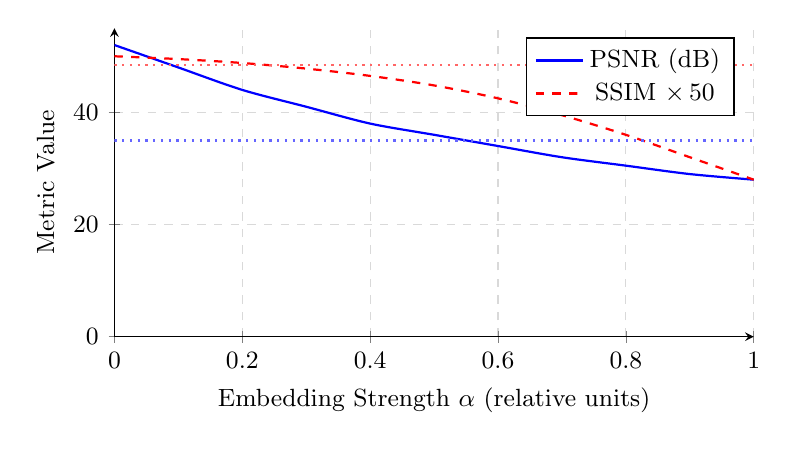
\begin{tikzpicture}
    \begin{axis}[
        width=0.80\textwidth, height=5.5cm,
        xlabel={Embedding Strength $\alpha$ (relative units)},
        ylabel={Metric Value},
        xmin=0, xmax=1.0,
        ymin=0, ymax=55,
        legend pos=north east,
        grid=major,
        grid style={dashed, gray!30},
        axis lines=left,
        tick label style={font=\small},
        label style={font=\small},
        legend style={font=\small},
      ]
      % PSNR curve (monotonically decreasing from ~52 to ~28)
      \addplot[thick, blue, smooth] coordinates {
        (0.0,52)(0.1,48)(0.2,44)(0.3,41)(0.4,38)(0.5,36)
        (0.6,34)(0.7,32)(0.8,30.5)(0.9,29)(1.0,28)
      };
      \addlegendentry{PSNR (dB)}

      % SSIM scaled to fit (multiply by 50 to show on same axis)
      \addplot[thick, red, dashed, smooth] coordinates {
        (0.0,50)(0.1,49.5)(0.2,48.8)(0.3,47.8)(0.4,46.5)(0.5,44.8)
        (0.6,42.5)(0.7,39.5)(0.8,36)(0.9,32)(1.0,28)
      };
      \addlegendentry{SSIM $\times\,50$}

      % Threshold lines
      \draw[dotted, thick, blue!60] (axis cs:0,35) -- (axis cs:1.0,35)
            node[right, font=\footnotesize, blue!60] {PSNR\,=\,35\,dB};
      \draw[dotted, thick, red!60]  (axis cs:0,48.5) -- (axis cs:1.0,48.5)
            node[right, font=\footnotesize, red!60]  {SSIM\,=\,0.97};
    \end{axis}
  \end{tikzpicture}
  \caption{Illustrative relationship between embedding strength $\alpha$ and the two
           imperceptibility metrics PSNR and SSIM (scaled by $50$). Both metrics decrease
           monotonically with increasing embedding strength. PSNR degrades rapidly even at
           moderate strengths, while SSIM is more tolerant of small-amplitude, high-frequency
           embedding signals that preserve structural content. This highlights the
           complementary nature of the two metrics.}
  \label{fig:psnr_ssim_tradeoff}
\end{figure}

\subsubsection{Relationship Between Imperceptibility Metrics}

Although PSNR and SSIM are both imperceptibility metrics, they capture different aspects of
image quality and can sometimes disagree on the ranking of steganographic methods. Embedding
in the low-frequency components of an image (e.g.\ the DC coefficients of DCT) produces large
intensity shifts that severely degrade PSNR but may preserve structural correlations and
therefore maintain a relatively high SSIM. Conversely, high-frequency noise-like embeddings
may produce a high PSNR (because energy is spread thinly across many pixels) while destroying
textural structures and yielding a low SSIM. This complementarity explains why both metrics
are reported in Chapter~5 and why neither alone provides a complete picture of imperceptibility.

% ----------------------------------------------------------
\subsection{Robustness Metrics}
\label{subsec:robustness_metrics}
% ----------------------------------------------------------

Robustness metrics quantify the ability of a steganographic system to recover the hidden
message after the stego-image has been subjected to signal processing or geometric attacks.
The two metrics used in this work are the Bit Error Rate (BER) and the Normalised Correlation
(NC).

\subsubsection{Bit Error Rate (BER)}

The Bit Error Rate is the primary robustness metric in steganography and digital communications
\cite{proakis2008digital}. It measures the fraction of payload bits that are incorrectly
recovered after extraction from a (possibly degraded) stego-image. Formally, let
$M = [m_1, m_2, \ldots, m_K]$ be the original binary message of length $K$ bits, and let
$\hat{M} = [\hat{m}_1, \hat{m}_2, \ldots, \hat{m}_K]$ be the extracted message after attack.
The BER is defined as:
%
\begin{equation}
  \mathrm{BER}(M,\, \hat{M}) = \frac{1}{K} \sum_{k=1}^{K} \mathbf{1}\bigl[\hat{m}_k \neq m_k\bigr],
  \label{eq:ber}
\end{equation}
%
where $\mathbf{1}[\cdot]$ is the indicator function that equals $1$ if its argument is true and
$0$ otherwise. The BER is a dimensionless quantity in the range $[0, 1]$, typically expressed
as a percentage or in scientific notation.

\paragraph{Interpretation and thresholds.}
%
\begin{itemize}
  \item $\mathrm{BER} = 0.0$ (or $0\%$): Perfect recovery; every bit of the hidden message is
        correctly extracted. This is the ideal outcome and is achievable only in the absence of
        attacks or with sufficiently powerful error correction coding.
  \item $\mathrm{BER} \leq 0.01$ ($\leq 1\%$): Excellent robustness; with appropriate error
        correction coding, the original message can be recovered reliably.
  \item $\mathrm{BER} \leq 0.05$ ($\leq 5\%$): Good robustness; recovery is possible with
        moderate ECC overhead.
  \item $\mathrm{BER} \approx 0.5$ ($\approx 50\%$): Complete failure; the extracted bits are
        no better than random, meaning the embedding has been entirely destroyed by the attack.
        This is the expected BER when attempting to extract a message from a cover image in
        which nothing was embedded.
\end{itemize}

\paragraph{Relationship to error correction coding.}
When the steganographic payload is protected by an error correction code with correction capacity
$t$ (i.e.\ the code can correct up to $t$ bit errors per codeword), perfect message recovery is
possible if and only if the BER satisfies:
%
\begin{equation}
  \mathrm{BER} < \frac{t}{n},
  \label{eq:ber_ecc}
\end{equation}
%
where $n$ is the codeword length. For example, a Reed-Solomon code with $n = 255$ and
$t = 31$ can correct up to $\approx 12.2\%$ BER. This relationship motivates the use of ECC
in the proposed framework and defines the BER budget available to the embedding and transmission
process.

\paragraph{BER under partial data loss.}
In the context of the present thesis, where the stego-image may be subjected to cropping or
localised tampering, the effective BER includes contributions from two distinct sources: (i)
signal-level errors caused by noise and compression in the surviving image regions, and (ii)
erasure errors caused by the complete removal of image regions containing embedded fragments.
These two error types require different mitigation strategies --- ECC for signal-level errors
and erasure codes or redundancy for erasure errors --- and are therefore tracked separately
in the experimental evaluation of Chapter~5.

\subsubsection{Normalised Correlation (NC)}

The Normalised Correlation provides an alternative measure of message recovery fidelity that is
more robust to systematic bit inversions than the raw BER. It is commonly used in digital
watermarking \cite{cox2007digital} and has been adopted in robust steganographic evaluation to
provide a continuous measure of recovery quality that degrades smoothly as attack intensity
increases. The NC between the original message $M$ and the extracted message $\hat{M}$, after
bipolar encoding ($0 \to -1$, $1 \to +1$), is defined as:
%
\begin{equation}
  \mathrm{NC}(M,\, \hat{M}) = \frac{1}{K}
    \sum_{k=1}^{K} \bar{m}_k \cdot \hat{\bar{m}}_k,
  \label{eq:nc}
\end{equation}
%
where $\bar{m}_k \in \{-1, +1\}$ and $\hat{\bar{m}}_k \in \{-1, +1\}$ are the bipolarly
encoded versions of the original and extracted bits, respectively.

\paragraph{Interpretation.}
%
\begin{itemize}
  \item $\mathrm{NC} = 1.0$: Perfect recovery; all bits agree.
  \item $\mathrm{NC} = 0.0$: Complete failure; extracted bits are uncorrelated with the
        original, as would occur if a random sequence were substituted.
  \item $\mathrm{NC} = -1.0$: All bits are inverted; this can occur under systematic polarity
        reversal attacks and would be incorrectly reported as BER $= 1.0$ (perfect failure) even
        though the message is recoverable by simple inversion. The NC captures this case.
\end{itemize}

The relationship between NC and BER for independently and identically distributed bit errors is:
%
\begin{equation}
  \mathrm{NC} = 1 - 2 \cdot \mathrm{BER},
  \label{eq:nc_ber_relationship}
\end{equation}
%
from which it follows that $\mathrm{BER} = 0$ corresponds to $\mathrm{NC} = 1$ and
$\mathrm{BER} = 0.5$ corresponds to $\mathrm{NC} = 0$. Both metrics therefore convey the same
information for independent errors, but NC is preferable when systematic errors or polarity
reversals are possible. In this work, both metrics are reported to facilitate comparison with
results from the watermarking literature, which predominantly uses NC.

% ----------------------------------------------------------
\subsection{Partial Recovery Rate (PRR)}
\label{subsec:prr}
% ----------------------------------------------------------

Classical steganographic evaluation is concerned with binary outcomes: either the entire message
is recovered (BER $\approx 0$) or it is not. In the context of the self-recovering framework
proposed in this thesis, however, the system is explicitly designed to recover \emph{partial}
messages when not all embedded fragments survive. A metric that captures this partial-recovery
behaviour is therefore needed.

We define the \textbf{Partial Recovery Rate (PRR)} as the fraction of payload fragments that
are successfully recovered (with BER below a threshold $\epsilon$ for each fragment) from the
degraded stego-image:
%
\begin{equation}
  \mathrm{PRR} = \frac{|\{i : \mathrm{BER}(F_i, \hat{F}_i) \leq \epsilon\}|}{N_F},
  \label{eq:prr}
\end{equation}
%
where $N_F$ is the total number of fragments in the structured payload, $F_i$ is the $i$-th
original fragment, $\hat{F}_i$ is the extracted version, and $\epsilon$ is a per-fragment BER
threshold (typically $0.05$ when ECC is applied at the fragment level). A PRR of $1.0$ indicates
complete recovery; a PRR of $0.5$ indicates that half the message fragments were correctly
extracted; a PRR of $0.0$ indicates total failure. This metric is unique to the present work
and is reported in Chapter~5 to assess the partial-recovery performance of the proposed framework
under cropping and localised tampering attacks.

% ----------------------------------------------------------
\subsection{Unified View of Evaluation Criteria}
\label{subsec:unified_view}
% ----------------------------------------------------------

Figure~\ref{fig:metrics_overview} provides a visual overview of the relationship between the
evaluation metrics defined in this section and the three steganographic objectives.

\begin{figure}[htbp]
  \centering
  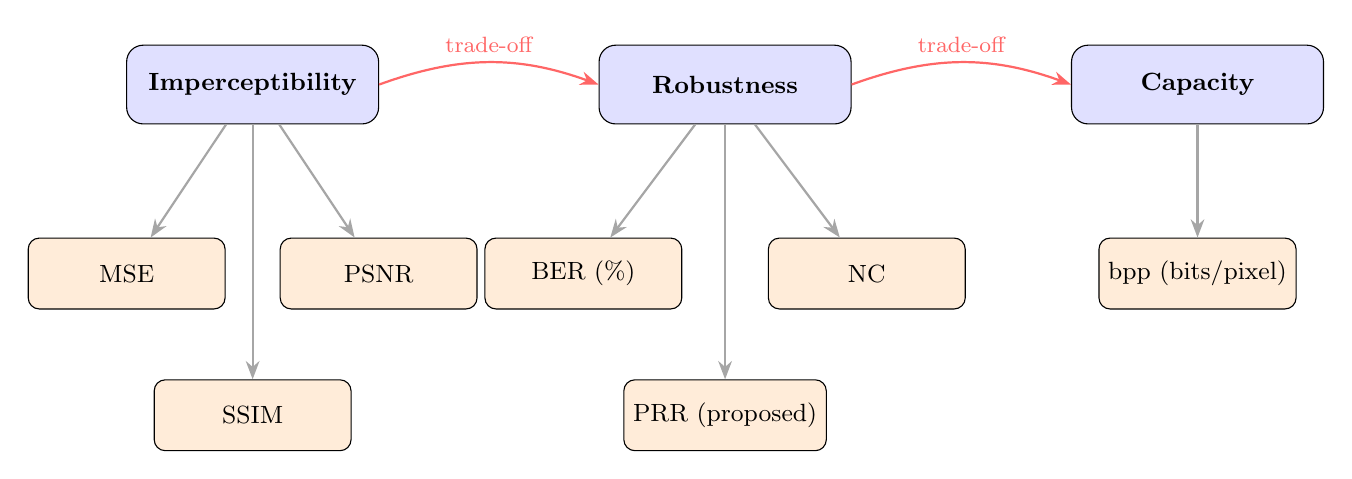
\begin{tikzpicture}[
      >=Stealth,
      obj/.style={draw, rounded corners=6pt, fill=blue!12,
                  minimum width=3.2cm, minimum height=1.0cm, align=center, font=\small\bfseries},
      met/.style={draw, rounded corners=4pt, fill=orange!15,
                  minimum width=2.5cm, minimum height=0.9cm, align=center, font=\small},
      arr/.style={->, thick, gray!70}
    ]
    % --- Objectives row ---
    \node[obj] (imp) at (0,0)    {Imperceptibility};
    \node[obj] (rob) at (6,0)    {Robustness};
    \node[obj] (cap) at (12,0)   {Capacity};

    % --- Metrics under Imperceptibility ---
    \node[met] (mse)  at (-1.6,-2.4) {MSE};
    \node[met] (psnr) at ( 1.6,-2.4) {PSNR};
    \node[met] (ssim) at ( 0,  -4.2) {SSIM};

    % --- Metrics under Robustness ---
    \node[met] (ber) at (4.2,-2.4)  {BER (\%)};
    \node[met] (nc)  at (7.8,-2.4)  {NC};
    \node[met] (prr) at (6,  -4.2)  {PRR (proposed)};

    % --- Metric under Capacity ---
    \node[met] (bpp) at (12,-2.4)   {bpp (bits/pixel)};

    % --- Downward arrows ---
    \draw[arr] (imp) -- (mse);
    \draw[arr] (imp) -- (psnr);
    \draw[arr] (imp) -- (ssim);
    \draw[arr] (rob) -- (ber);
    \draw[arr] (rob) -- (nc);
    \draw[arr] (rob) -- (prr);
    \draw[arr] (cap) -- (bpp);

    % --- Trade-off arrows between objectives ---
    \draw[->, thick, red!60]
      (imp.east) to[bend left=20]
      node[above, font=\footnotesize, red!60]{trade-off} (rob.west);
    \draw[->, thick, red!60]
      (rob.east) to[bend left=20]
      node[above, font=\footnotesize, red!60]{trade-off} (cap.west);

  \end{tikzpicture}
  \caption{Relationship between the three steganographic objectives and the quantitative
           evaluation metrics used in this thesis. The trade-offs between objectives
           are captured by tracking all metrics simultaneously across experimental conditions.
           PRR (Partial Recovery Rate) is a metric introduced in this work to assess the
           unique partial-recovery capability of the proposed framework.}
  \label{fig:metrics_overview}
\end{figure}

Table~\ref{tab:metrics_summary} summarises all evaluation metrics, their definitions, their
measurement units, and the performance thresholds adopted in this thesis.

\begin{table}[htbp]
  \centering
  \caption{Summary of evaluation metrics used in this thesis. Thresholds represent
           commonly accepted standards in the steganographic and image quality literature.}
  \label{tab:metrics_summary}
  \renewcommand{\arraystretch}{1.35}
  \small
  \begin{tabular}{@{} l l l c l @{}}
    \toprule
    \textbf{Metric} & \textbf{Objective} & \textbf{Formula} & \textbf{Range}
                    & \textbf{Good threshold} \\
    \midrule
    MSE  & Imperceptibility & $\frac{1}{MN}\sum(C-S)^2$ & $[0, \infty)$ & As small as possible \\
    PSNR & Imperceptibility & $10\log_{10}(L^2/\mathrm{MSE})$ & $(0, \infty)$ dB & $> 35$\,dB \\
    SSIM & Imperceptibility & Eq.~\eqref{eq:ssim} & $[-1,\,1]$ & $> 0.97$ \\
    \midrule
    BER  & Robustness & $\frac{1}{K}\sum \mathbf{1}[\hat{m}\neq m]$ & $[0,\,1]$ & $< 0.05$ \\
    NC   & Robustness & $\frac{1}{K}\sum \bar{m}\cdot\hat{\bar{m}}$ & $[-1,\,1]$ & $> 0.9$ \\
    PRR  & Partial recovery & Eq.~\eqref{eq:prr} & $[0,\,1]$ & $> 0.7$ (proposed) \\
    \midrule
    bpp  & Capacity & bits embedded per pixel & $(0,\,8]$ & Application-dependent \\
    \bottomrule
  \end{tabular}
\end{table}

These metrics, taken together, provide a comprehensive and multi-dimensional assessment of
steganographic performance. In Chapter~5, each metric is reported for the proposed framework
and for the classical baselines under each attack scenario, enabling a rigorous comparative
evaluation that respects the multi-objective nature of the steganographic design problem.

 %=================================

\chapter{Proposed Self-Recovering Steganography Framework}

\section{Design Motivation and Objectives}
This chapter introduces the proposed steganographic framework, which is designed to address the limitations identified in the literature review, particularly the fragility of conventional embedding methods under severe image degradation and geometric desynchronization.

The primary design goal of the proposed framework is to enhance payload survivability rather than solely reinforcing embedding locations. Unlike traditional approaches that assume intact data and perfect synchronization, the proposed system explicitly assumes partial data loss and uncontrolled image transformations. The framework is therefore designed to tolerate damage, enable partial recovery, and reconstruct missing information using structured payload relationships.

\section{High-Level System Overview}
This section presents a conceptual overview of the proposed framework, illustrating the main processing stages at both the sender and receiver sides.

At a high level, the system consists of four main components:
\begin{itemize}
    \item Payload structuring and self-description
    \item Fragmentation and inter-fragment relationship encoding
    \item Multi-domain embedding strategy
    \item Damage-aware extraction and reconstruction
\end{itemize}

The interaction between these components enables robust message recovery even when a significant portion of the embedded data is degraded or removed.

\subsection{Sender-Side Processing Pipeline}
The sender-side pipeline begins with the secret message and produces a stego-image suitable for transmission through uncontrolled digital environments.

The main stages include:
\begin{itemize}
    \item Conversion of the secret message into a structured payload
    \item Fragment generation and relationship encoding
    \item Selection of embedding domains and regions
    \item Embedding of fragments into the cover image
\end{itemize}

\subsection{Receiver-Side Processing Pipeline}
The receiver-side pipeline operates on a potentially degraded stego-image and attempts to recover the original message.

The extraction process includes:
\begin{itemize}
    \item Detection and extraction of embedded fragments
    \item Damage estimation and fragment confidence evaluation
    \item Fragment validation and relationship checking
    \item Partial reconstruction and message reassembly
\end{itemize}

\section{Structured Payload Representation}
Instead of embedding raw binary data, the proposed framework transforms the secret message into a self-describing structured payload. This payload contains not only the original message bits but also additional information that enables validation, ordering, and reconstruction.

\subsection{Payload Components}
Each payload fragment contains the following elements:
\begin{itemize}
    \item Fragment identifier and ordering information
    \item Local payload data
    \item Lightweight checksum for integrity verification
    \item Cross-fragment reference information
\end{itemize}

This structure allows individual fragments to contribute to the reconstruction of missing or corrupted fragments.

\subsection{Inter-Fragment Relationships}
Fragments are not treated as independent entities. Instead, each fragment stores partial information about neighboring and non-neighboring fragments. These relationships form a redundancy graph that supports reconstruction under partial data loss.

The use of relational information enables recovery even when contiguous regions of the image are destroyed.

\section{Fragmentation Strategy}
The structured payload is divided into multiple interconnected fragments to increase resilience against localized damage.

\subsection{Fragment Size and Granularity}
Fragment size is chosen as a compromise between robustness and capacity. Smaller fragments improve survivability under cropping, while larger fragments reduce overhead.

This work adopts a fixed fragment size to simplify reconstruction and evaluation.

\subsection{Redundancy and Distribution Policy}
Controlled redundancy is introduced at the fragment level rather than the bit level. Each fragment is embedded multiple times across different domains or image regions according to a predefined distribution policy.

The redundancy level is configurable and directly impacts robustness and payload capacity.

\section{Multi-Domain Embedding Strategy}
To reduce vulnerability to specific attack types, fragments are embedded across multiple embedding domains, each offering resistance to different forms of degradation.

\subsection{Spatial Domain Embedding}
Fragments embedded in spatial texture regions are resilient to localized cropping and partial tampering. Texture-based masking is used to minimize visual distortion.

\subsection{Frequency Domain Embedding}
Mid-frequency DCT coefficients are used to embed fragments resistant to JPEG compression and moderate noise. Embedding strength is adjusted to balance imperceptibility and robustness.

\subsection{Multi-Scale and Redundant Embedding}
Selected fragments are embedded at different spatial resolutions or downsampled representations of the image to improve resilience against resizing operations.

\subsection{Color Channel Utilization}
For color images, redundancy is introduced across luminance and chrominance channels. Stronger embedding is applied to the luminance channel, while weaker redundant embedding is used in chrominance channels.

\section{Embedding Control and Parameter Selection}
This section describes the parameters governing embedding strength, fragment placement, and redundancy levels.

\subsection{Key-Based Fragment Placement}
A secret key is used to pseudo-randomly determine fragment locations and embedding domains, enhancing security and preventing unauthorized extraction.

\subsection{Embedding Strength Adaptation}
Embedding strength is adjusted based on local image characteristics, such as texture intensity and frequency stability.

\section{Damage-Aware Extraction Process}
Unlike traditional extraction schemes, the proposed framework does not assume intact data. Instead, it explicitly estimates damage and adapts the extraction process accordingly.

\subsection{Fragment Detection and Validation}
Extracted fragments are validated using checksums and structural consistency checks. Invalid or severely corrupted fragments are discarded or assigned low confidence.

\subsection{Confidence Scoring Mechanism}
Each fragment is assigned a confidence score based on extraction quality, consistency with neighboring fragments, and agreement with relational information.

\subsection{Adaptive Fragment Selection}
Fragments with higher confidence scores are prioritized during reconstruction. Lower-confidence fragments are used only when necessary.

\section{Message Reconstruction and Self-Recovery}
The final message is reconstructed using surviving fragments and their encoded relationships.

\subsection{Partial Reconstruction Strategy}
Missing fragments are reconstructed using relational summaries and redundancy information provided by neighboring fragments.

\subsection{Failure Conditions}
This section defines conditions under which full or partial recovery is not possible, such as excessive data loss or severe compound attacks.

\section{Computational Complexity and Practical Considerations}
The computational overhead of the proposed framework is analyzed in terms of embedding time, extraction time, and memory requirements.

\subsection{Complexity Analysis}
The complexity of payload structuring, embedding, and extraction is discussed qualitatively.

\subsection{Implementation Constraints}
Practical limitations related to image size, payload capacity, and real-world deployment are identified.

\section{Summary of the Proposed Framework}
This section summarizes the key design principles and highlights how the proposed framework addresses the research gaps identified in Chapter 2, particularly synchronization loss, partial data destruction, and robustness under compound attacks.


% =========================

\chapter{Implementation and Experimental Setup}
\section{Development Environment}
The tools and software environment used for implementation are described.

\section{Dataset Description}
The image datasets used for experimentation are presented.

\section{Attack Simulation}
This section describes how image degradation and tampering scenarios are simulated.

\section{Evaluation Metrics}
\subsection{Imperceptibility Metrics}
PSNR and SSIM are introduced.

\subsection{Robustness Metrics}
Bit Error Rate (BER) and Normalized Correlation (NC) are defined.

% =========================

\chapter{Results and Discussion}
\section{Imperceptibility Evaluation}
Visual quality and distortion analysis are presented.

\section{Robustness Under Image Degradation}
Performance under compression, noise, and resizing is analyzed.

\section{Robustness Under Partial Data Loss}
The impact of cropping and localized tampering is evaluated.
 
\section{Comparative Analysis}
The proposed framework is compared with classical steganography methods.

\section{Discussion of Results}
Strengths, weaknesses, and observed trade-offs are discussed.

% =========================

\chapter{Conclusion and Future Work}
\section{Summary of Findings}
The main outcomes of the study are summarized.

\section{Limitations}
Practical and theoretical limitations of the framework are discussed.

\section{Future Research Directions}
Possible extensions and improvements are suggested.

\bibliographystyle{unsrt}
\bibliography{references}

\end{document}
